\documentclass[titlepage,11pt]{article}
\usepackage{enumitem}
\usepackage{listings}
\usepackage{amsmath}
\usepackage{graphicx}
\usepackage[font=small,labelfont=bf]{caption}
\usepackage[bahasa]{babel}
\usepackage{float}
\usepackage{verbatim}
\usepackage{graphicx,tabularx,multirow}
\usepackage{xcolor}
\usepackage[onehalfspacing]{setspace}
\usepackage[
	allcolors=visigrey,
	colorlinks=true,
]{hyperref}
\usepackage[a4paper,left=2cm,right=2cm]{geometry}

%Code listing style pak akok
\definecolor{codegreen}{rgb}{0,0.6,0}
\definecolor{codegray}{rgb}{0.5,0.5,0.5}
\definecolor{codepurple}{rgb}{0.58,0,0.82}
\definecolor{backcolour}{rgb}{0.95,0.95,0.92}

\lstdefinestyle{mystyle}{
	backgroundcolor=\color{backcolour}, commentstyle=\color{codegreen},
	keywordstyle=\color{magenta},
	numberstyle=\small\color{codegray},
	stringstyle=\color{codepurple},
	basicstyle=\ttfamily\footnotesize,
	breakatwhitespace=false,         
	breaklines=true,                 
	captionpos=t,                    
	keepspaces=true,                 
	numbers=left,                    
	numbersep=5pt,                  
	showspaces=false,                
	showstringspaces=false,
	showtabs=false,           
	frame = single,
	tabsize=2
}
\lstset{style=mystyle}

\definecolor{visigrey}{rgb}{.1,.15,.15}
\geometry{top=1cm,bottom=.5cm}
\savegeometry{titlepage}
\geometry{top=2cm,bottom=2cm}
\savegeometry{main}

\def\bspace{\(\qquad\qquad\qquad\)}
\usepackage[T1]{fontenc}
\usepackage[utf8]{inputenc}
\usepackage{tgheros}
\renewcommand*\familydefault{\sfdefault}

\setcounter{tocdepth}{6}

\def\autor{Laboratorium }
\def\lab{Multimedia dan Internet of Things}
\def\departemen{Departemen Teknik Komputer}
\def\institut{Institut Teknologi Sepuluh Nopember}
\def\praktikum{Praktikum \\ Dasar Pemrograman}
% Ubah Judul sesuai dengan modul
\def\judul{Judul}
\def\tahun{2024}
\begin{document}
% Ubah Bahasa sesuai dengan keinginan
\selectlanguage{bahasa}
\input{Cover/Header.tex}
% Pilih Modul yang akan di build
% \section*{Tujuan}
\begin{itemize}[label=$\bullet$, itemsep=-1pt, leftmargin=*]
	%    \setlength\itemsep{0.5em}
	% \item Students are able to create projects on an IDE
	% \item Students can demonstrate his/her knowledge of the structure of a C program
	% \item Students can demonstrate his/her knowledge of C data types
	% \item Students can demonstrate his/her knowledge of C operators
	% \item Students are able to use function to read inputs from keyboard
	% \item Students are able to use function to print texts on screen
	\item Mahasiswa dapat membuat proyek di dalam IDE
	\item Mahasiswa dapat menunjukkan pengetahuan mereka tentang struktur program dalam bahasa C
	\item Mahasiswa dapat menunjukkan pengetahuan mereka tentang tipe data dalam bahasa C
	\item Mahasiswa dapat menunjukkan pengetahuan mereka tentang operator dalam bahasa C
	\item Mahasiswa mampu menggunakan fungsi untuk membaca masukan dari keyboard
	\item Mahasiswa mampu menggunakan fungsi untuk mencetak teks di layar

\end{itemize}
\section*{Mengenal Bahasa C}
Bahasa C adalah bahasa pemrograman tingkat menengah yang dikembangkan oleh Dennis Ritchie pada tahun 1972 di Bell Laboratories.
Disebut “tingkat menengah” karena C punya kemampuan dekat ke mesin (bisa mengakses memori langsung, pointer, dll.),
tetapi tetap memiliki struktur yang mudah dipahami layaknya bahasa tingkat tinggi.

\subsection*{Kenapa bahasa C penting?}
\begin{enumerate}
    \item \textbf{Dasar banyak bahasa modern} \\
    Bahasa C menjadi ``induk'' dari banyak bahasa lain, misalnya: C++, Java, C\#, Objective-C, bahkan Python terinspirasi oleh C.

    \item \textbf{Cepat \& efisien} \\
    Program dalam C biasanya lebih ringan dan cepat dibanding banyak bahasa lain, karena C berhubungan langsung dengan hardware.

    \item \textbf{Portabel (multi-platform)} \\
    Program C bisa dijalankan di berbagai sistem operasi (Windows, Linux, macOS, embedded system) hanya dengan sedikit penyesuaian.

    \item \textbf{Dipakai di sistem penting} \\
    Banyak sistem operasi (UNIX, Linux, Windows kernel), driver perangkat keras, compiler, bahkan game lama ditulis dengan C.
\end{enumerate}

\section*{IDE (Integrated Development Environment)}
IDE adalah singkatan dari "Integrated Development Environment" dalam bahasa Inggris.
Dalam Bahasa Indonesia, IDE dapat diterjemahkan menjadi "Lingkungan Pengembangan Terintegrasi" atau "Ruang Kerja Pengembangan Terpadu."
IDE adalah sebuah perangkat lunak yang dirancang untuk membantu pengembang perangkat lunak dalam proses pengembangan, pengkodean, dan pengujian aplikasi komputer.
\\
Berikut ini adalah daftar aplikasi IDE bahasa C yang dapat digunakan.
\begin{itemize}
	\item CodeBlocks
\end{itemize}
\section*{Membuat proyek baru pada IDE Code::Blocks}
\subsection*{Langkah untuk membuat proyek baru}
\begin{enumerate}
	\item Go to File $>$ New $>$ Project
	      \begin{figure}[H]
		      \centering
		      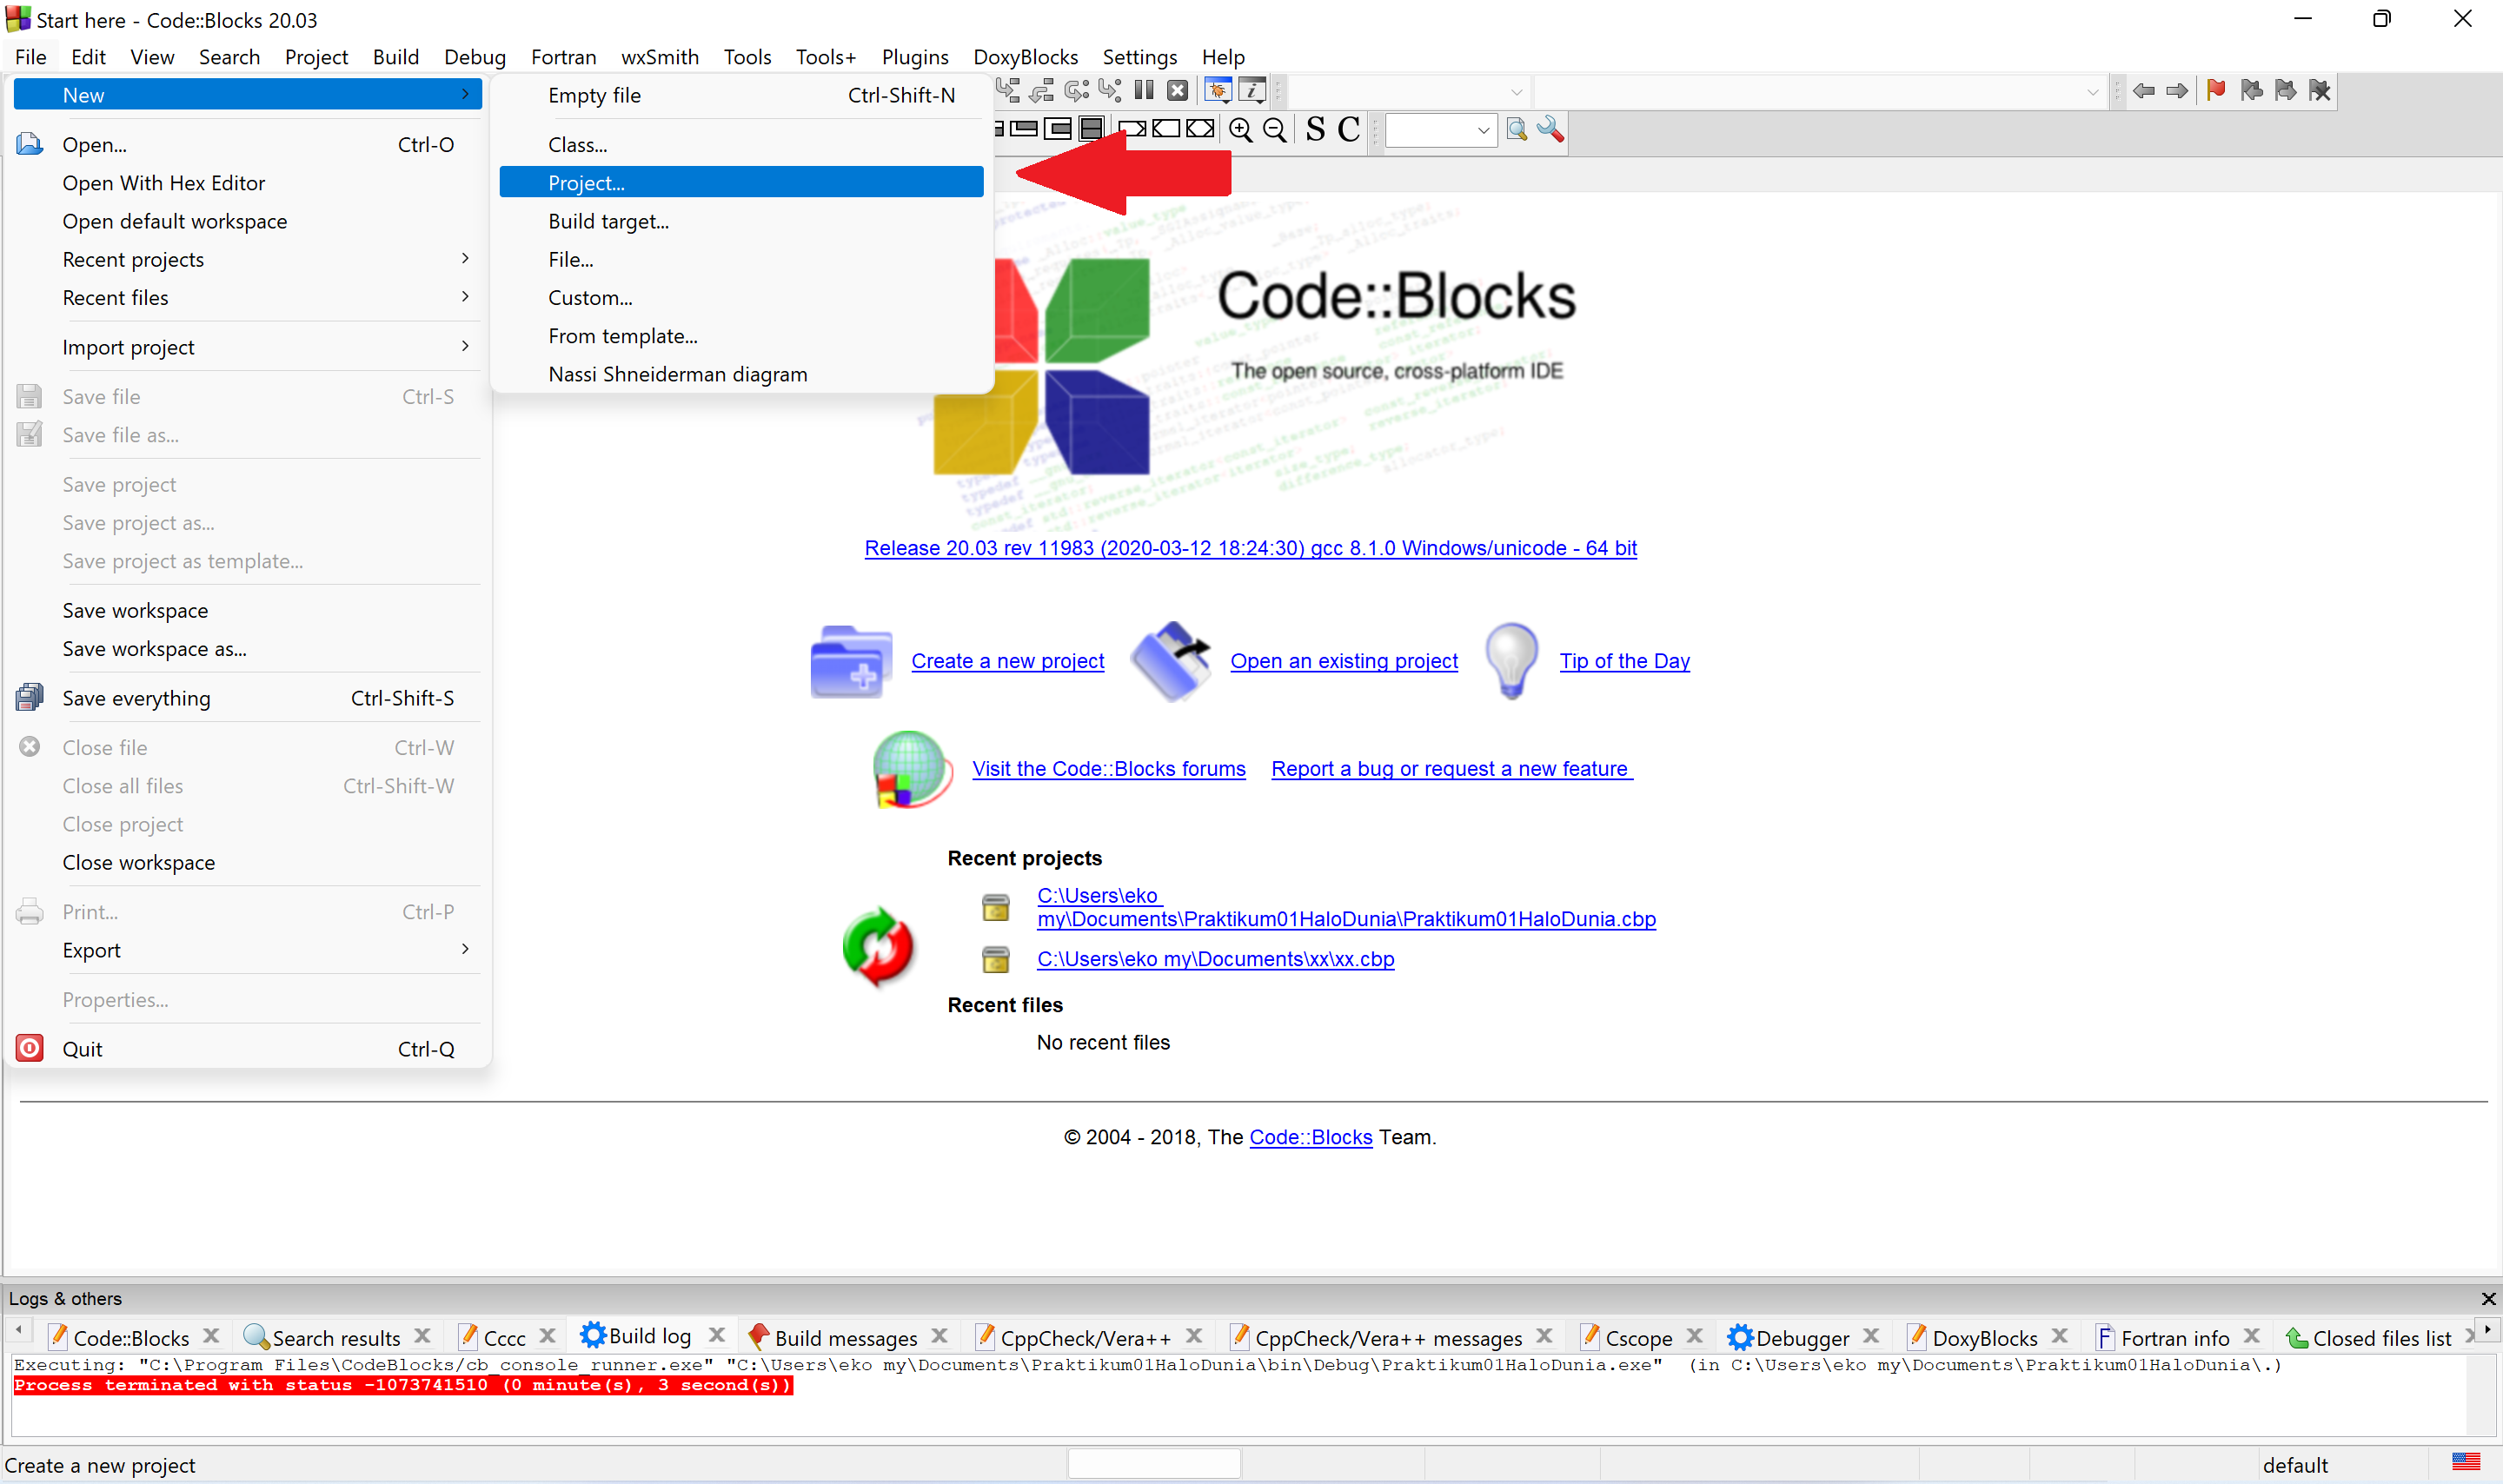
\includegraphics[width=0.7\linewidth]{P1/img/screenshot002.png}
		      \caption{}
		      \label{fig:screenshot002}
	      \end{figure}
	\item Klik Console Application
	      \begin{figure}[H]
		      \centering
		      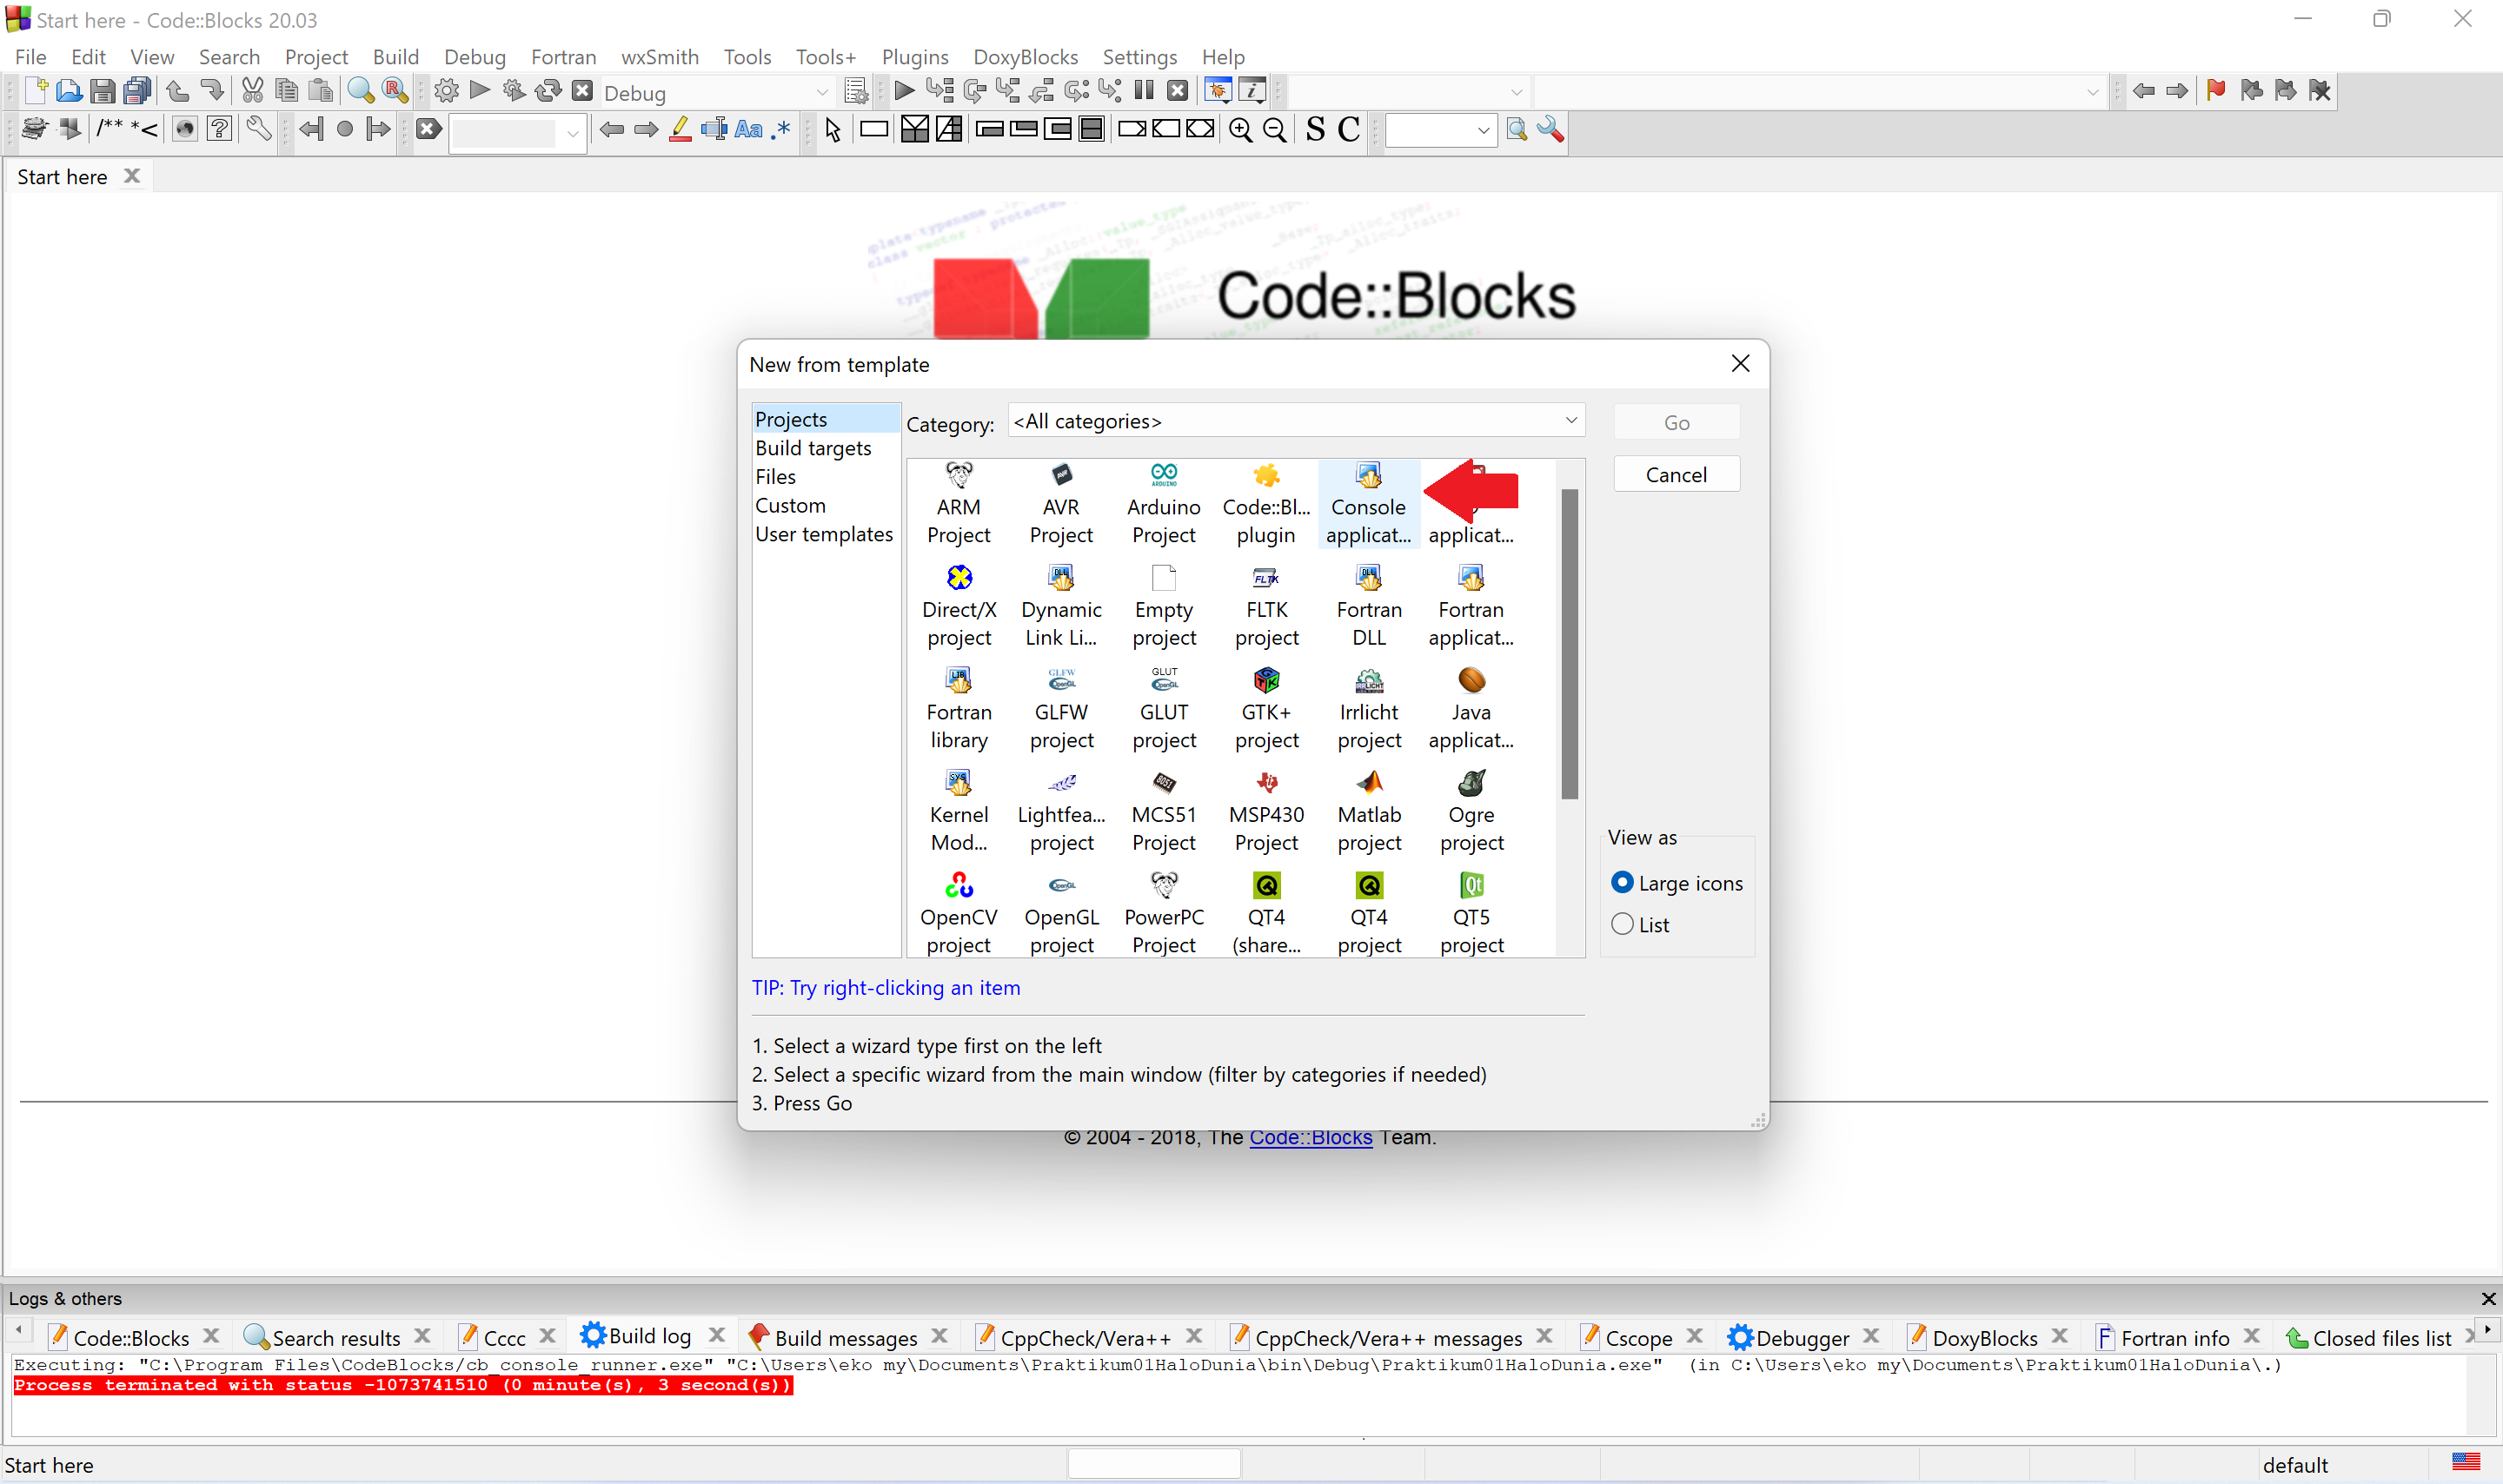
\includegraphics[width=0.7\linewidth]{P1/img/screenshot004.png}
		      \caption{}
		      \label{fig:screenshot004}
	      \end{figure}
	\item Pilih C sebagai bahasa Pemrograman
	      \begin{figure}[H]
		      \centering
		      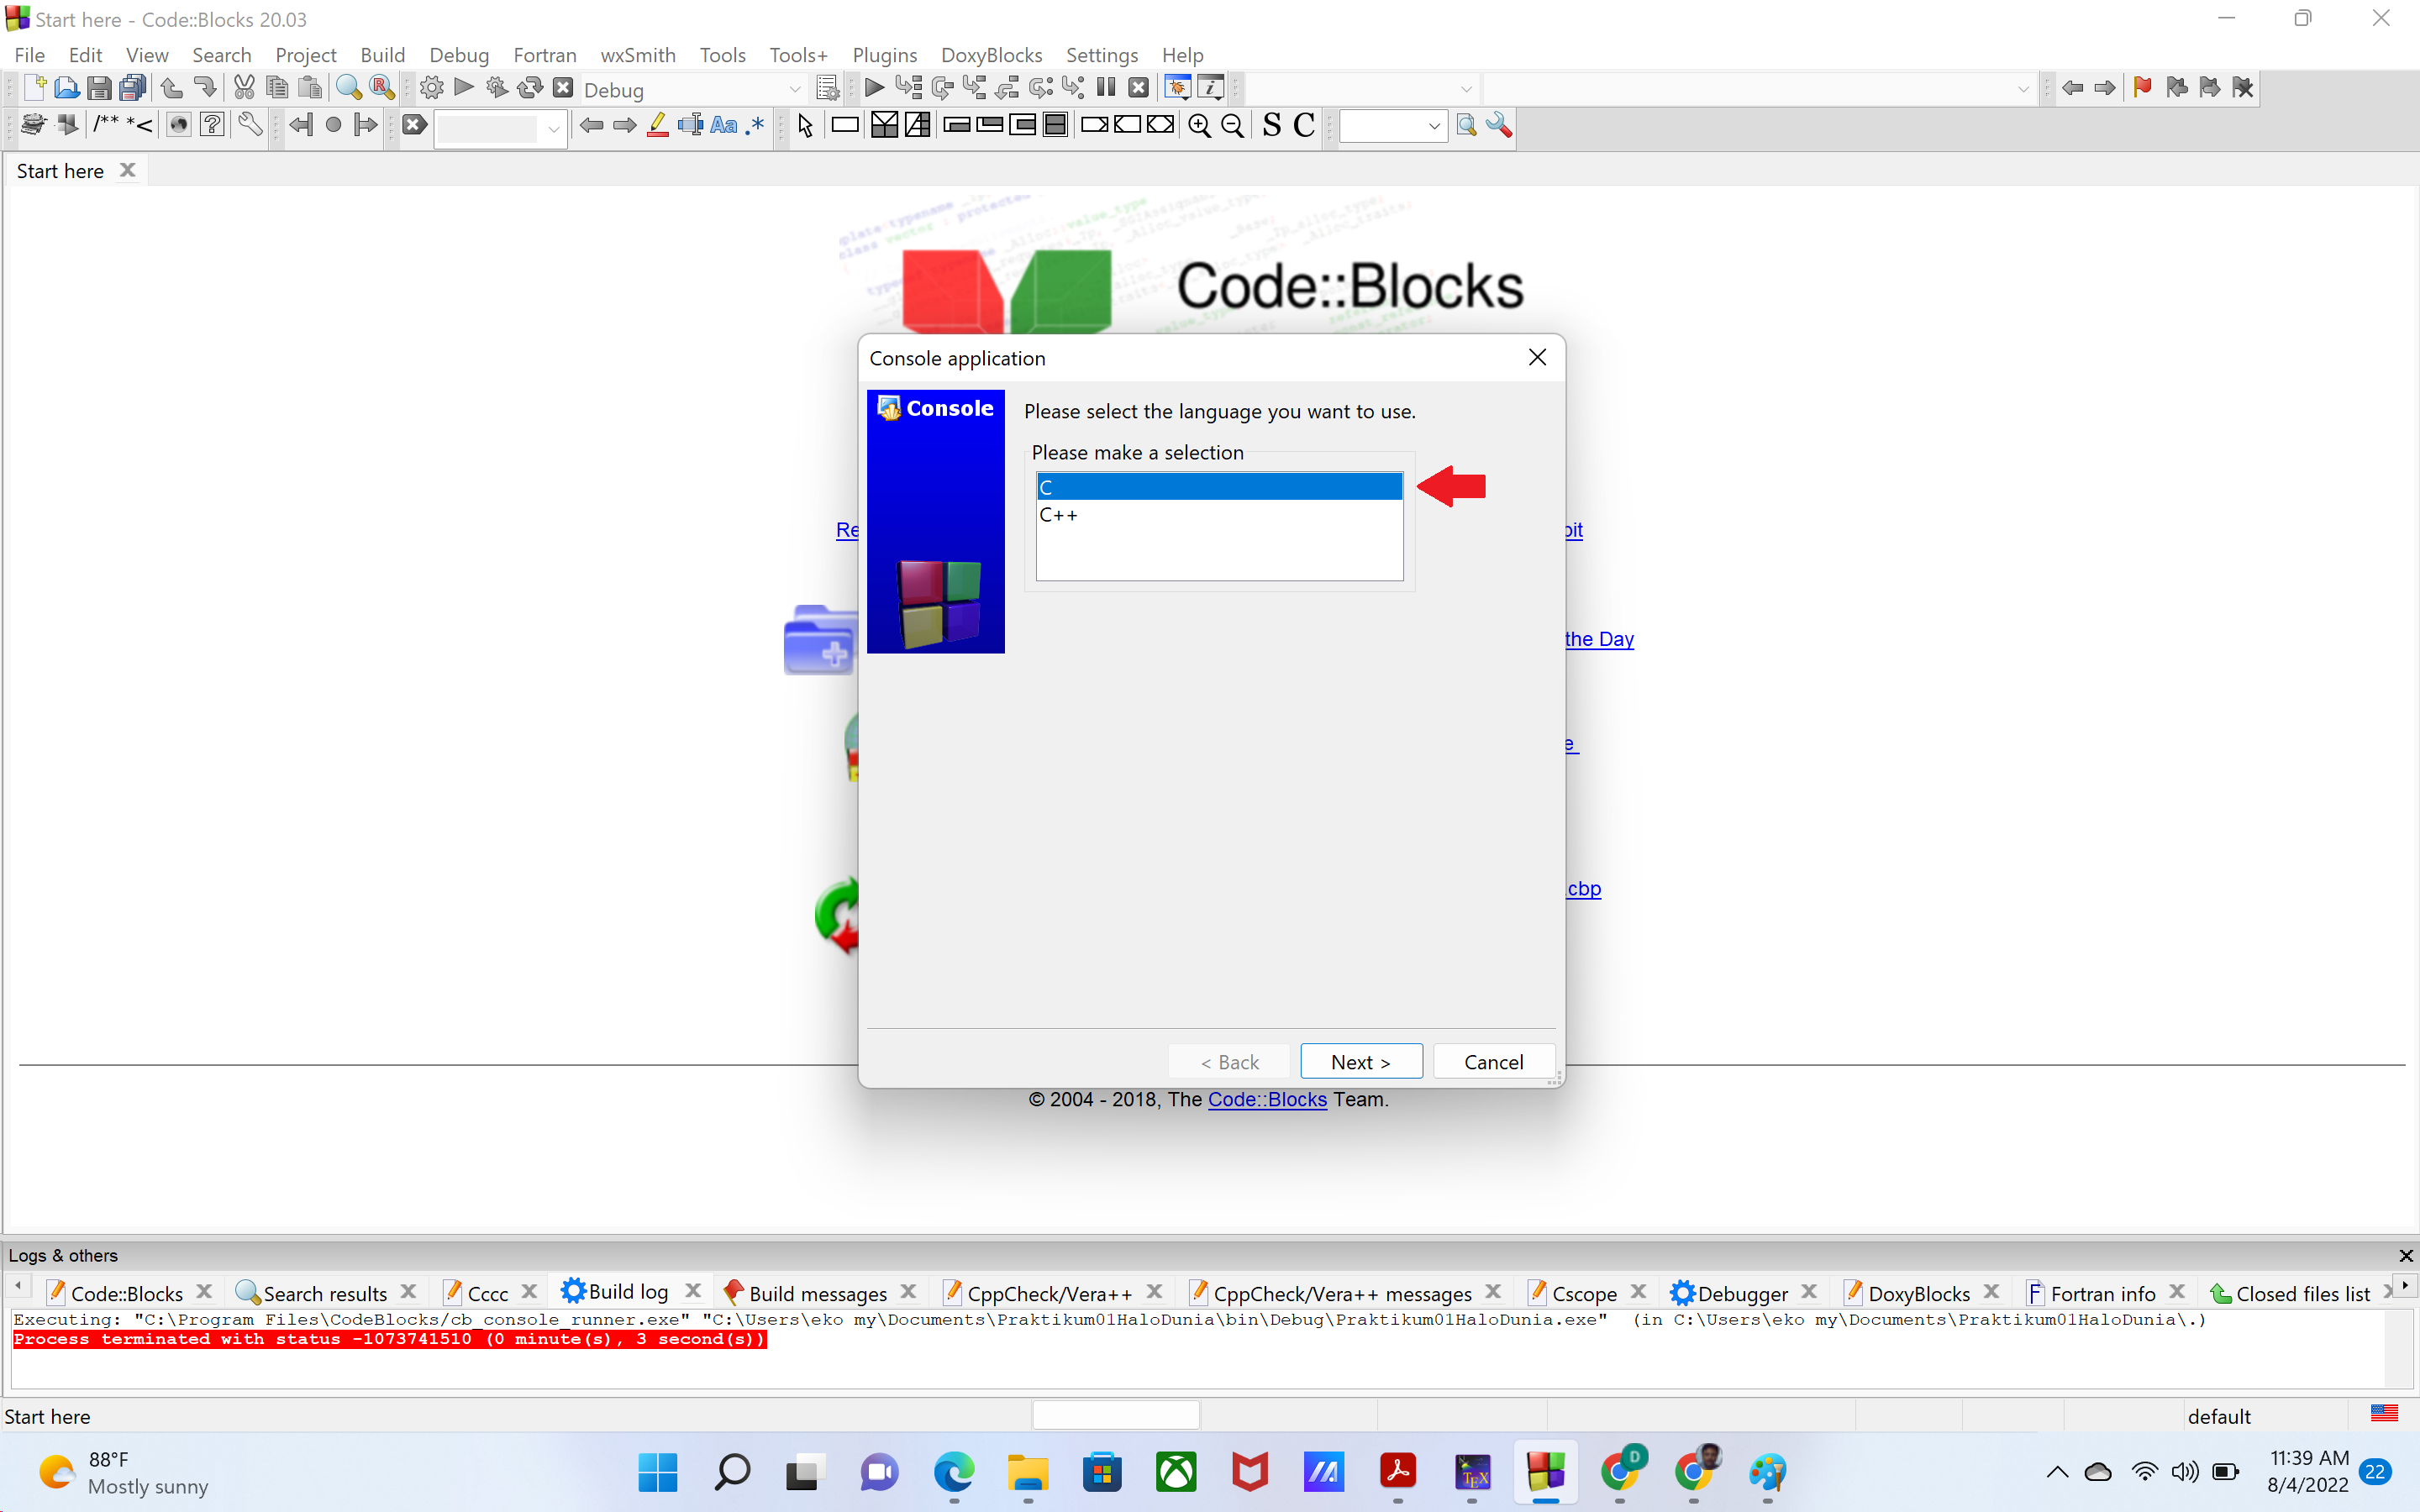
\includegraphics[width=0.7\linewidth]{P1/img/screenshot005.png}
		      \caption{}
		      \label{fig:screenshot005}
	      \end{figure}
	\item Berikan nama ke project
	      \begin{figure}[H]
		      \centering
		      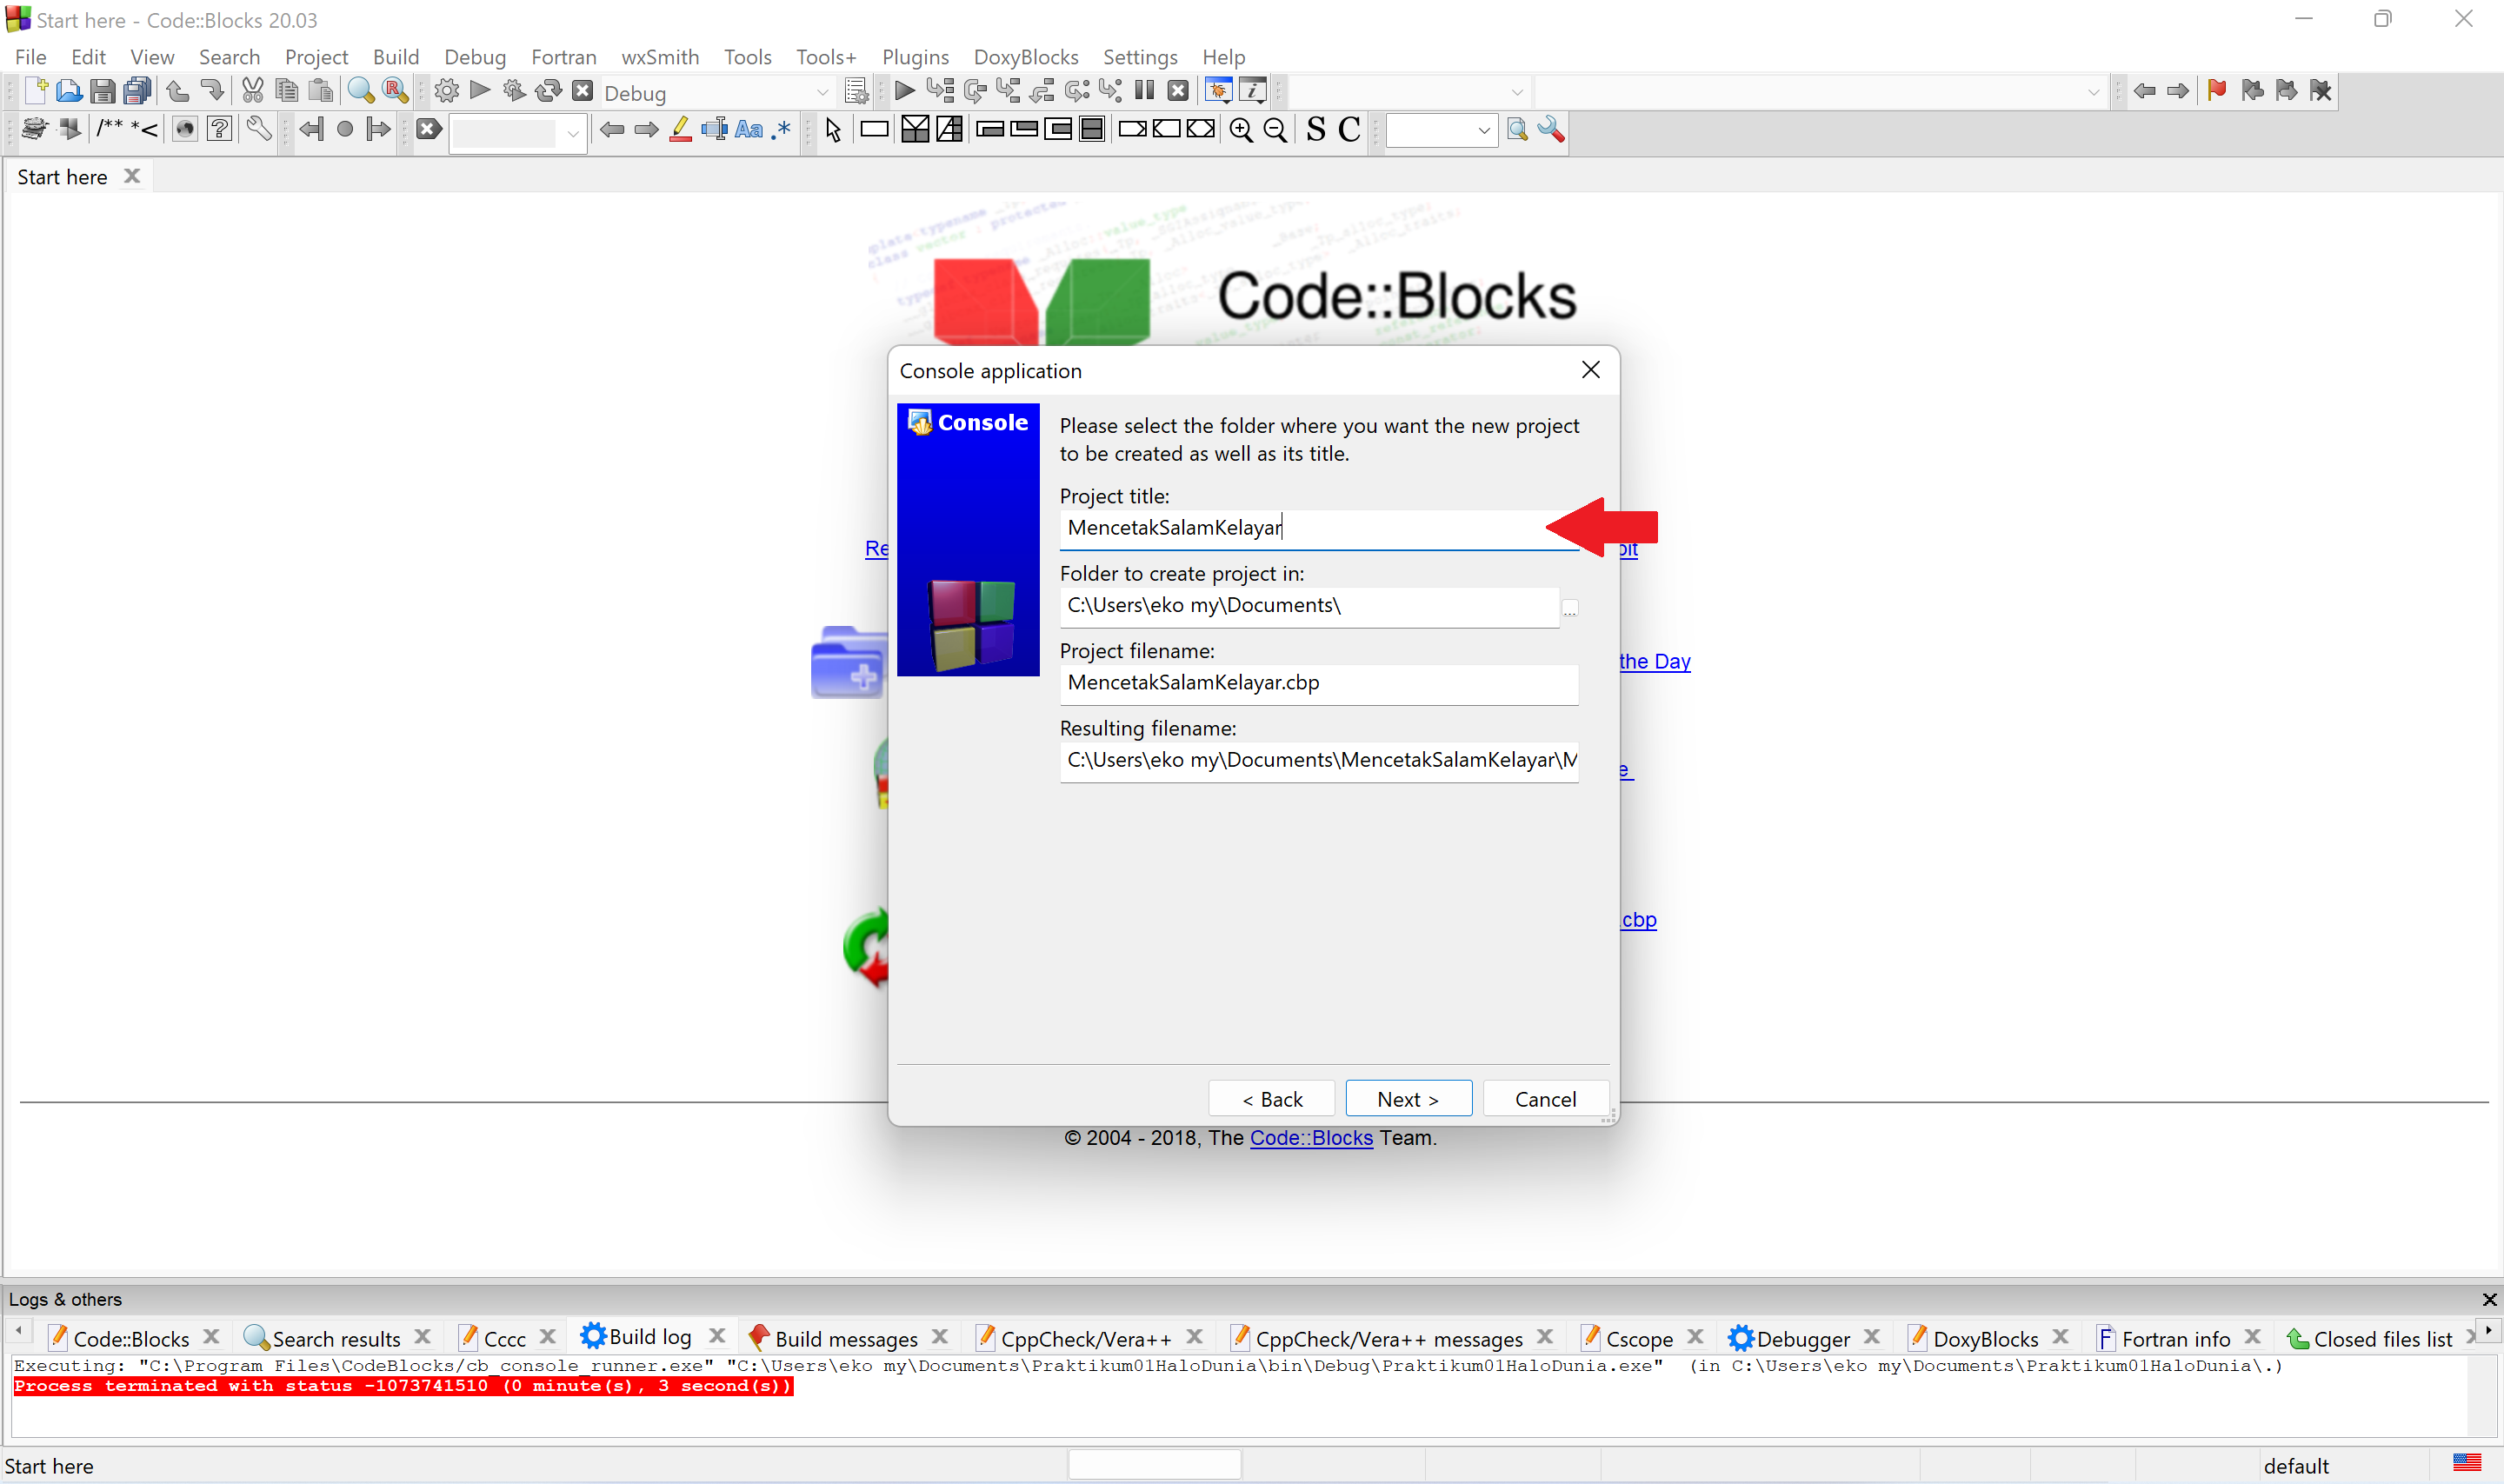
\includegraphics[width=0.7\linewidth]{P1/img/screenshot006.png}
		      \caption{}
		      \label{fig:screenshot006}
	      \end{figure}
	\item  Pilih compiler (gcc), pilih direktori untuk menyimpan, dan klik save.
	      \begin{figure}[H]
		      \centering
		      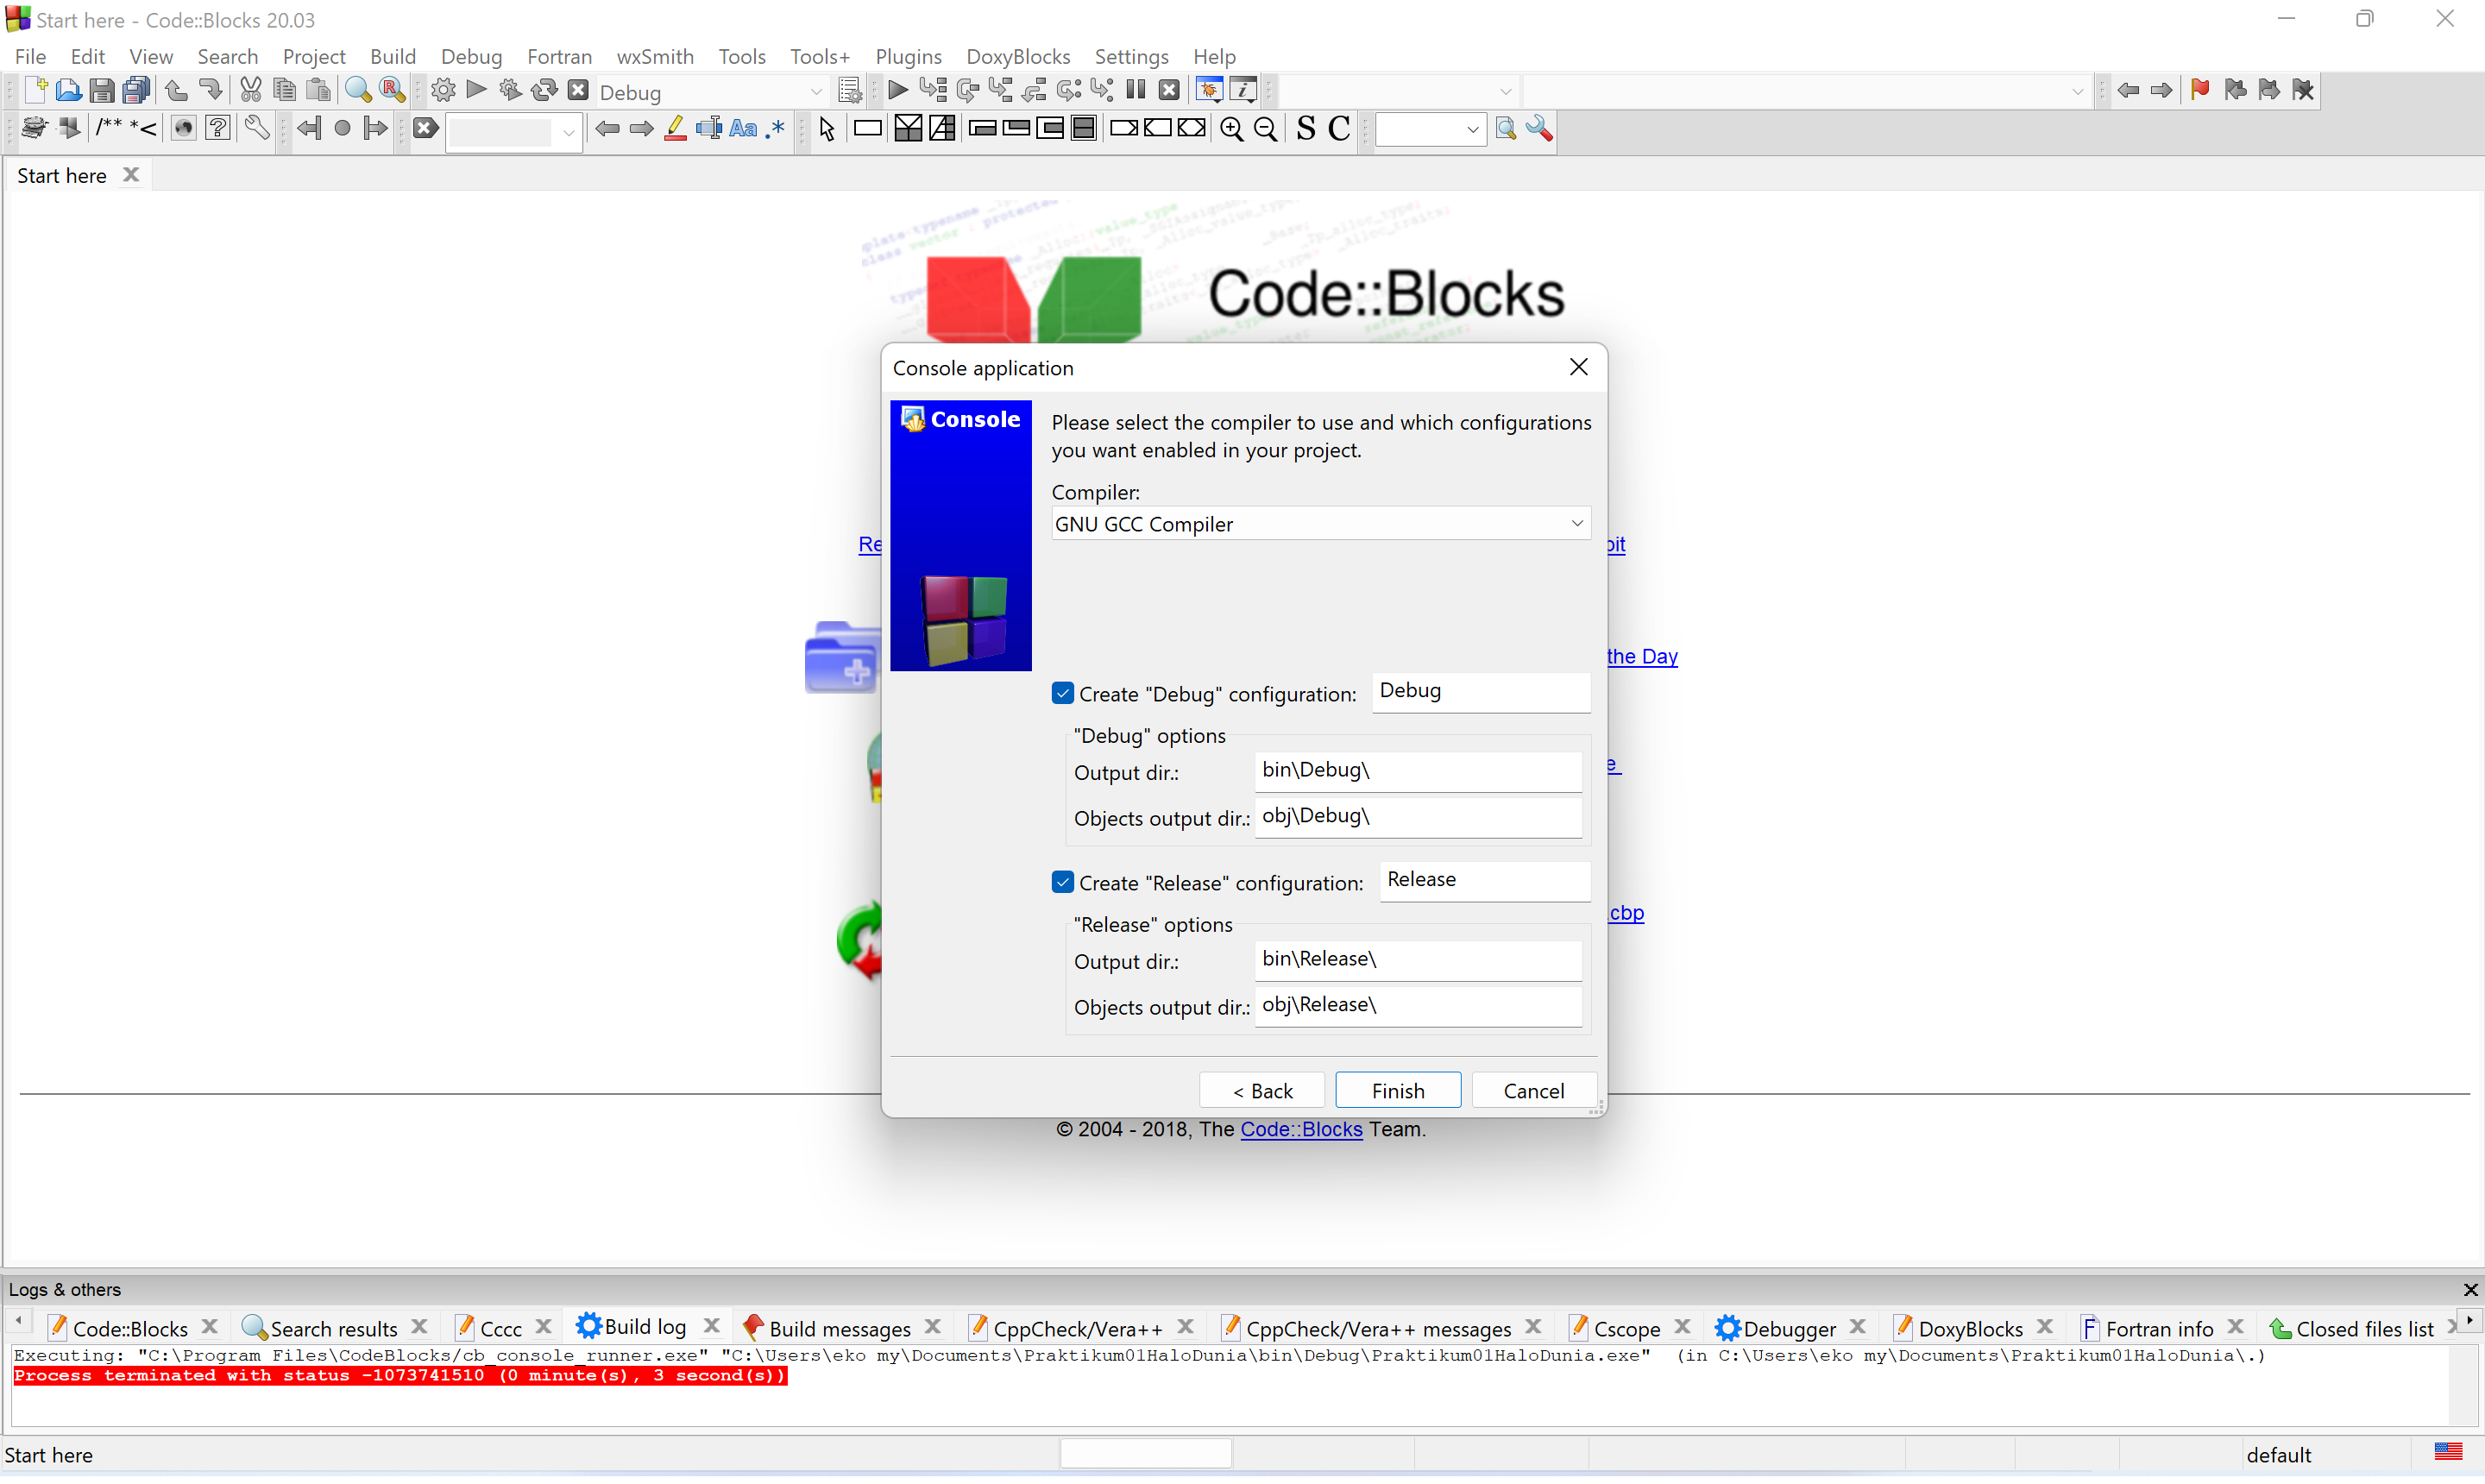
\includegraphics[width=0.7\linewidth]{P1/img/screenshot007.png}
		      \caption{}
		      \label{fig:screenshot007}
	      \end{figure}
	\item Ketikan kode pada Gambar\ref{fig:screenshot008} ke Code::Blocks
	      \begin{figure}[H]
		      \centering
		      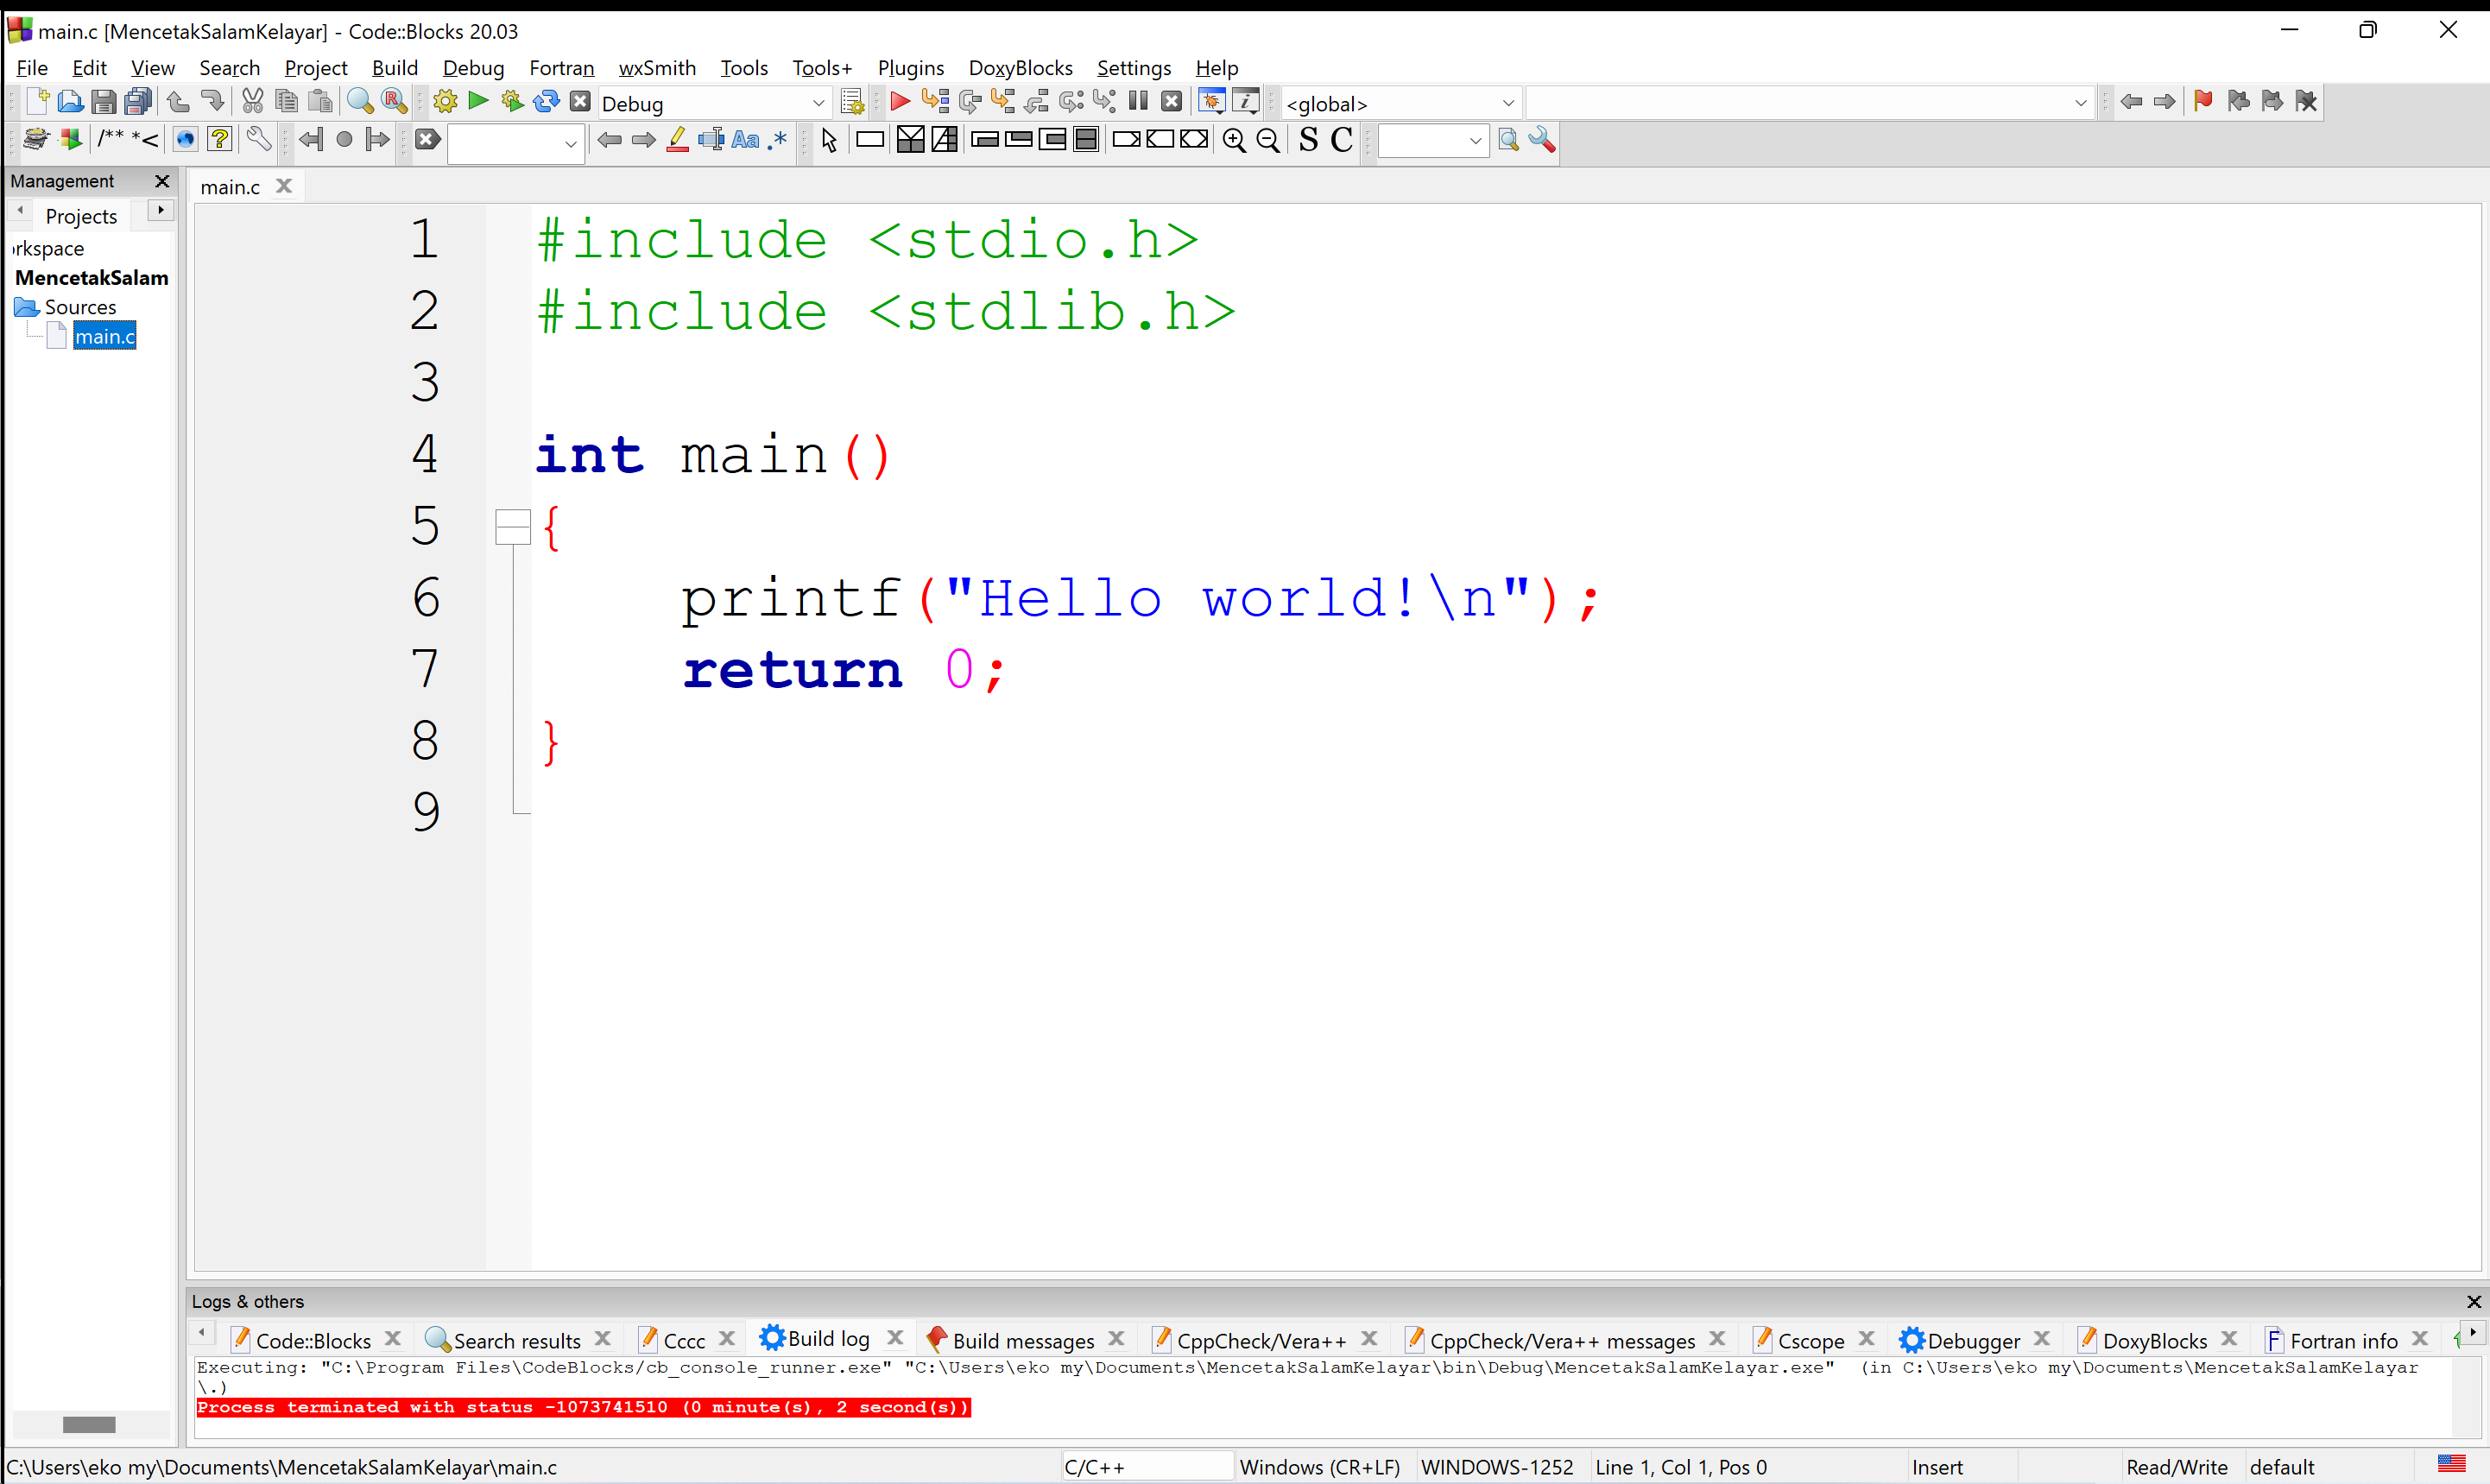
\includegraphics[width=0.7\linewidth]{P1/img/screenshot008.png}
		      \caption{}
		      \label{fig:screenshot008}
	      \end{figure}
	\item Klik Build$->$Build and Run atau tekan F9
	      \begin{figure}[H]
		      \centering
		      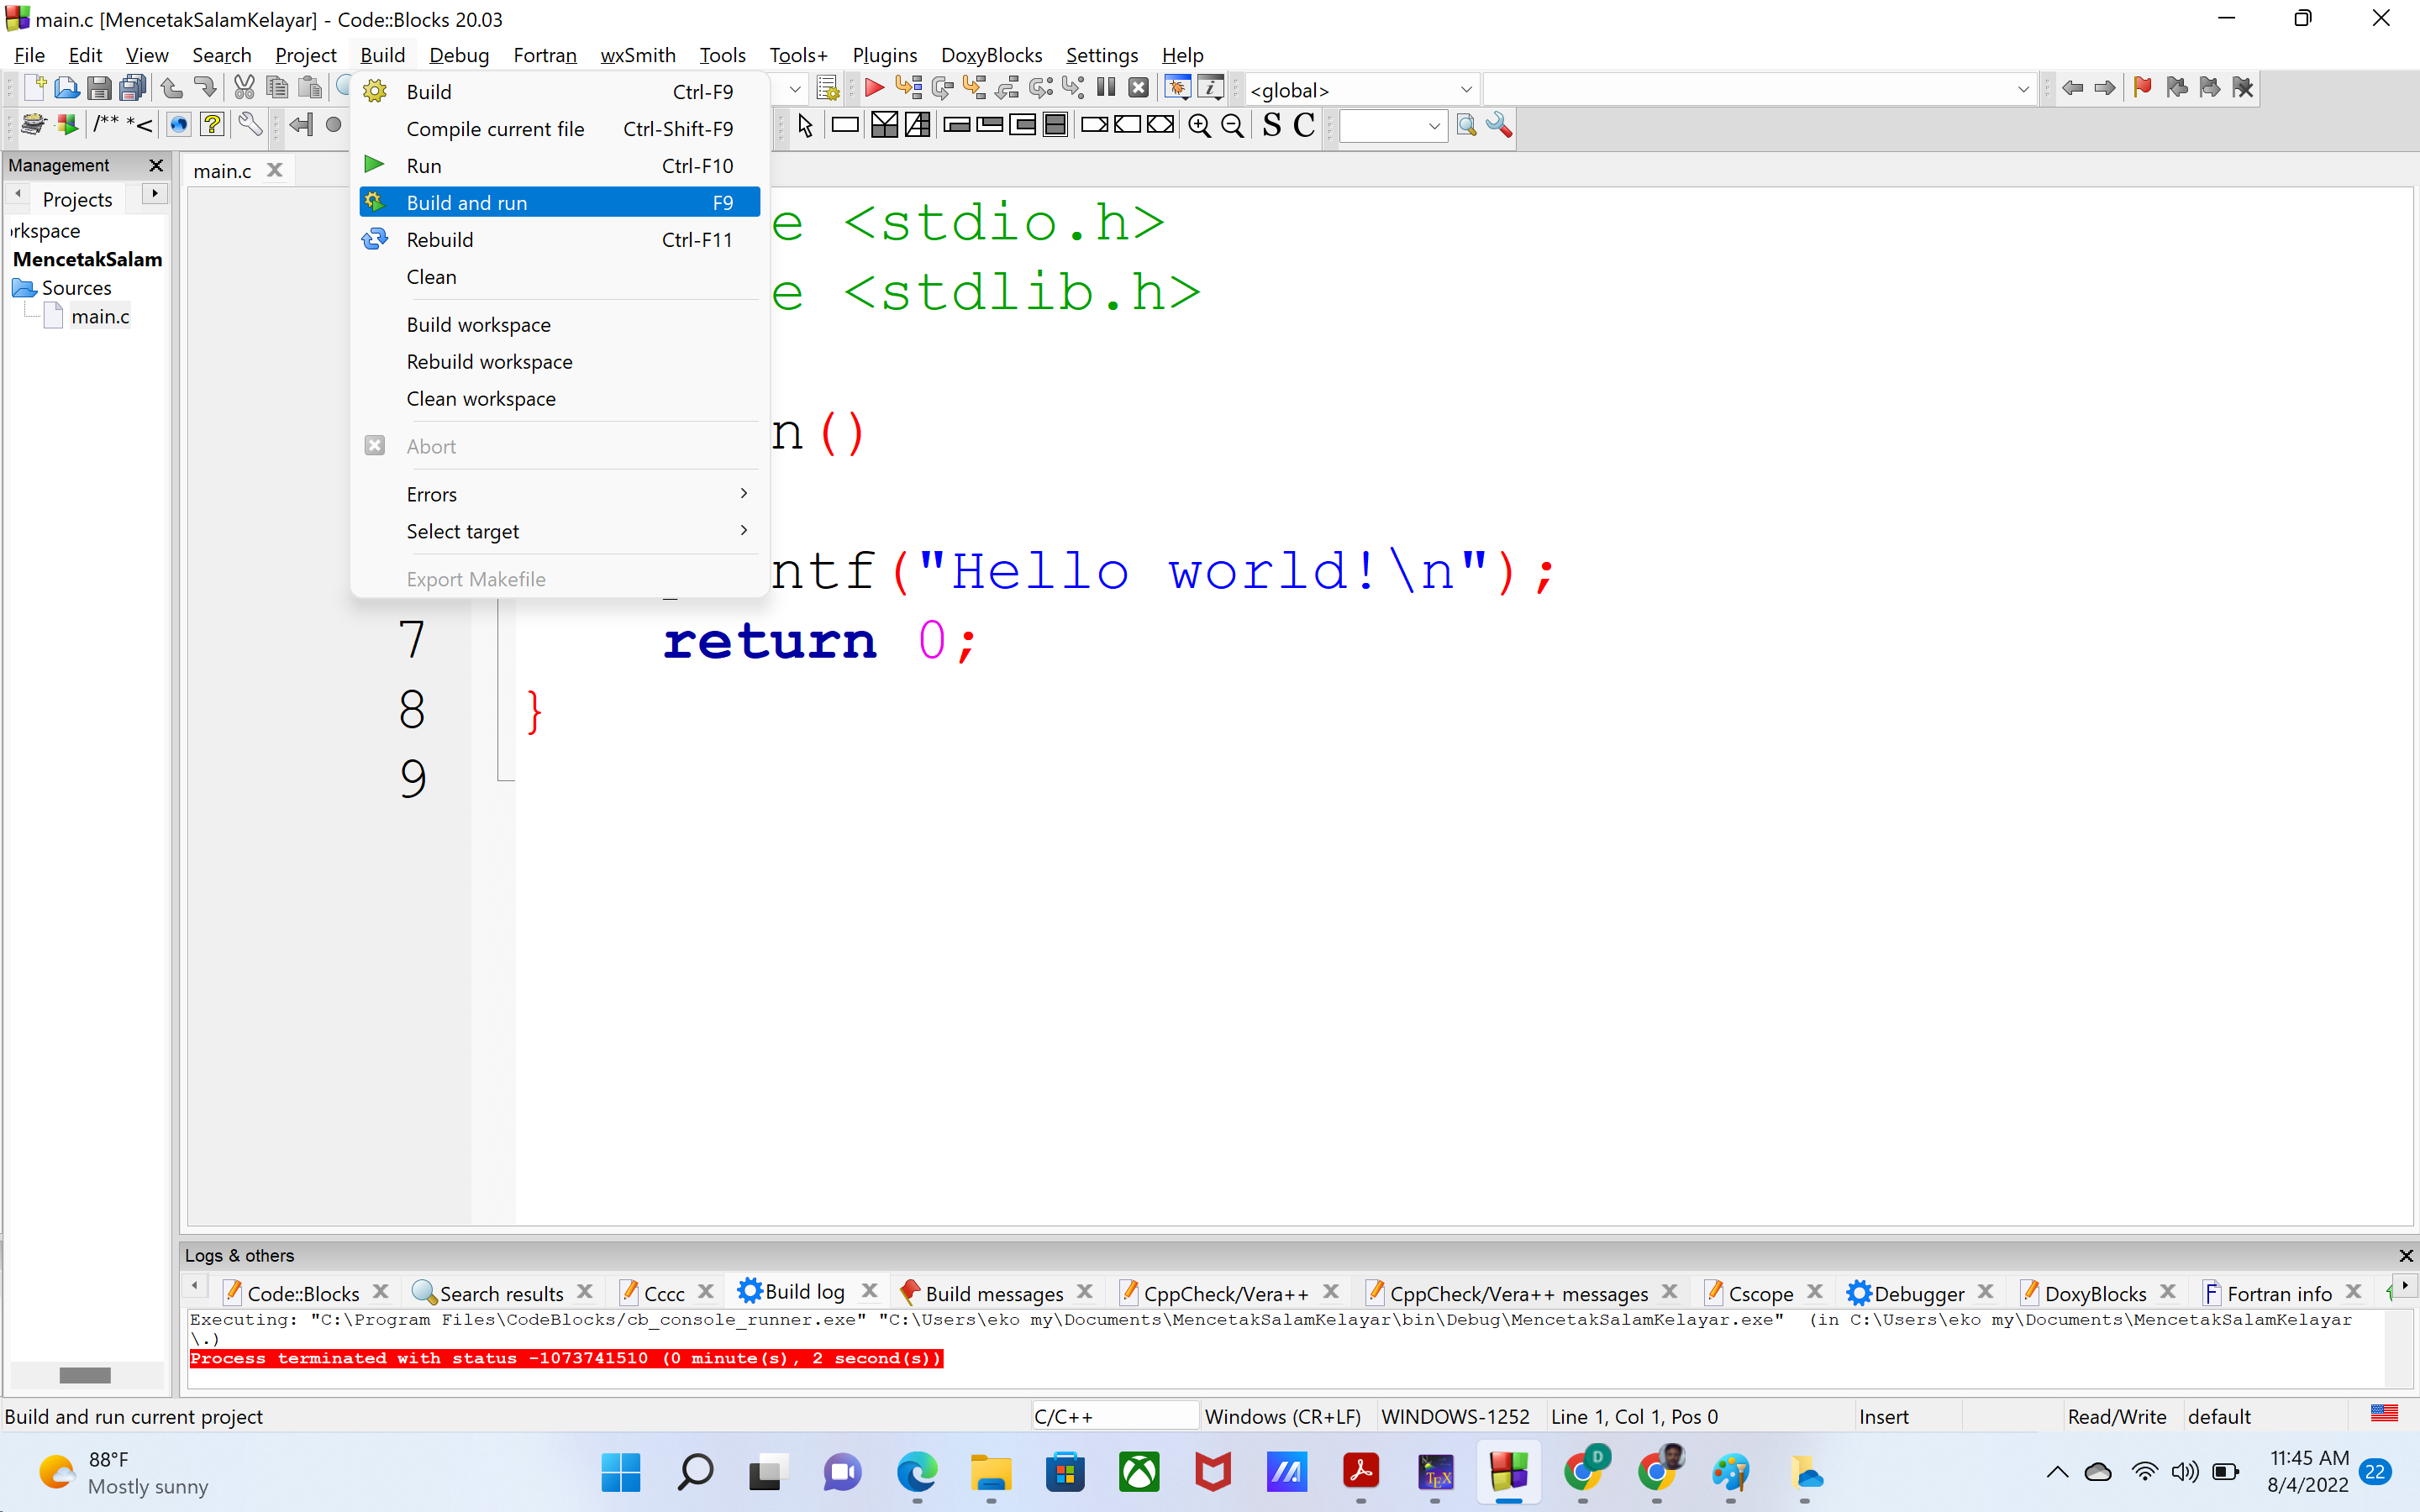
\includegraphics[width=0.7\linewidth]{P1/img/screenshot009.png}
		      \caption{}
		      \label{fig:screenshot009}
	      \end{figure}
	\item Keluaran dari program dapat dilihat di console
	      \begin{figure}[H]
		      \centering
		      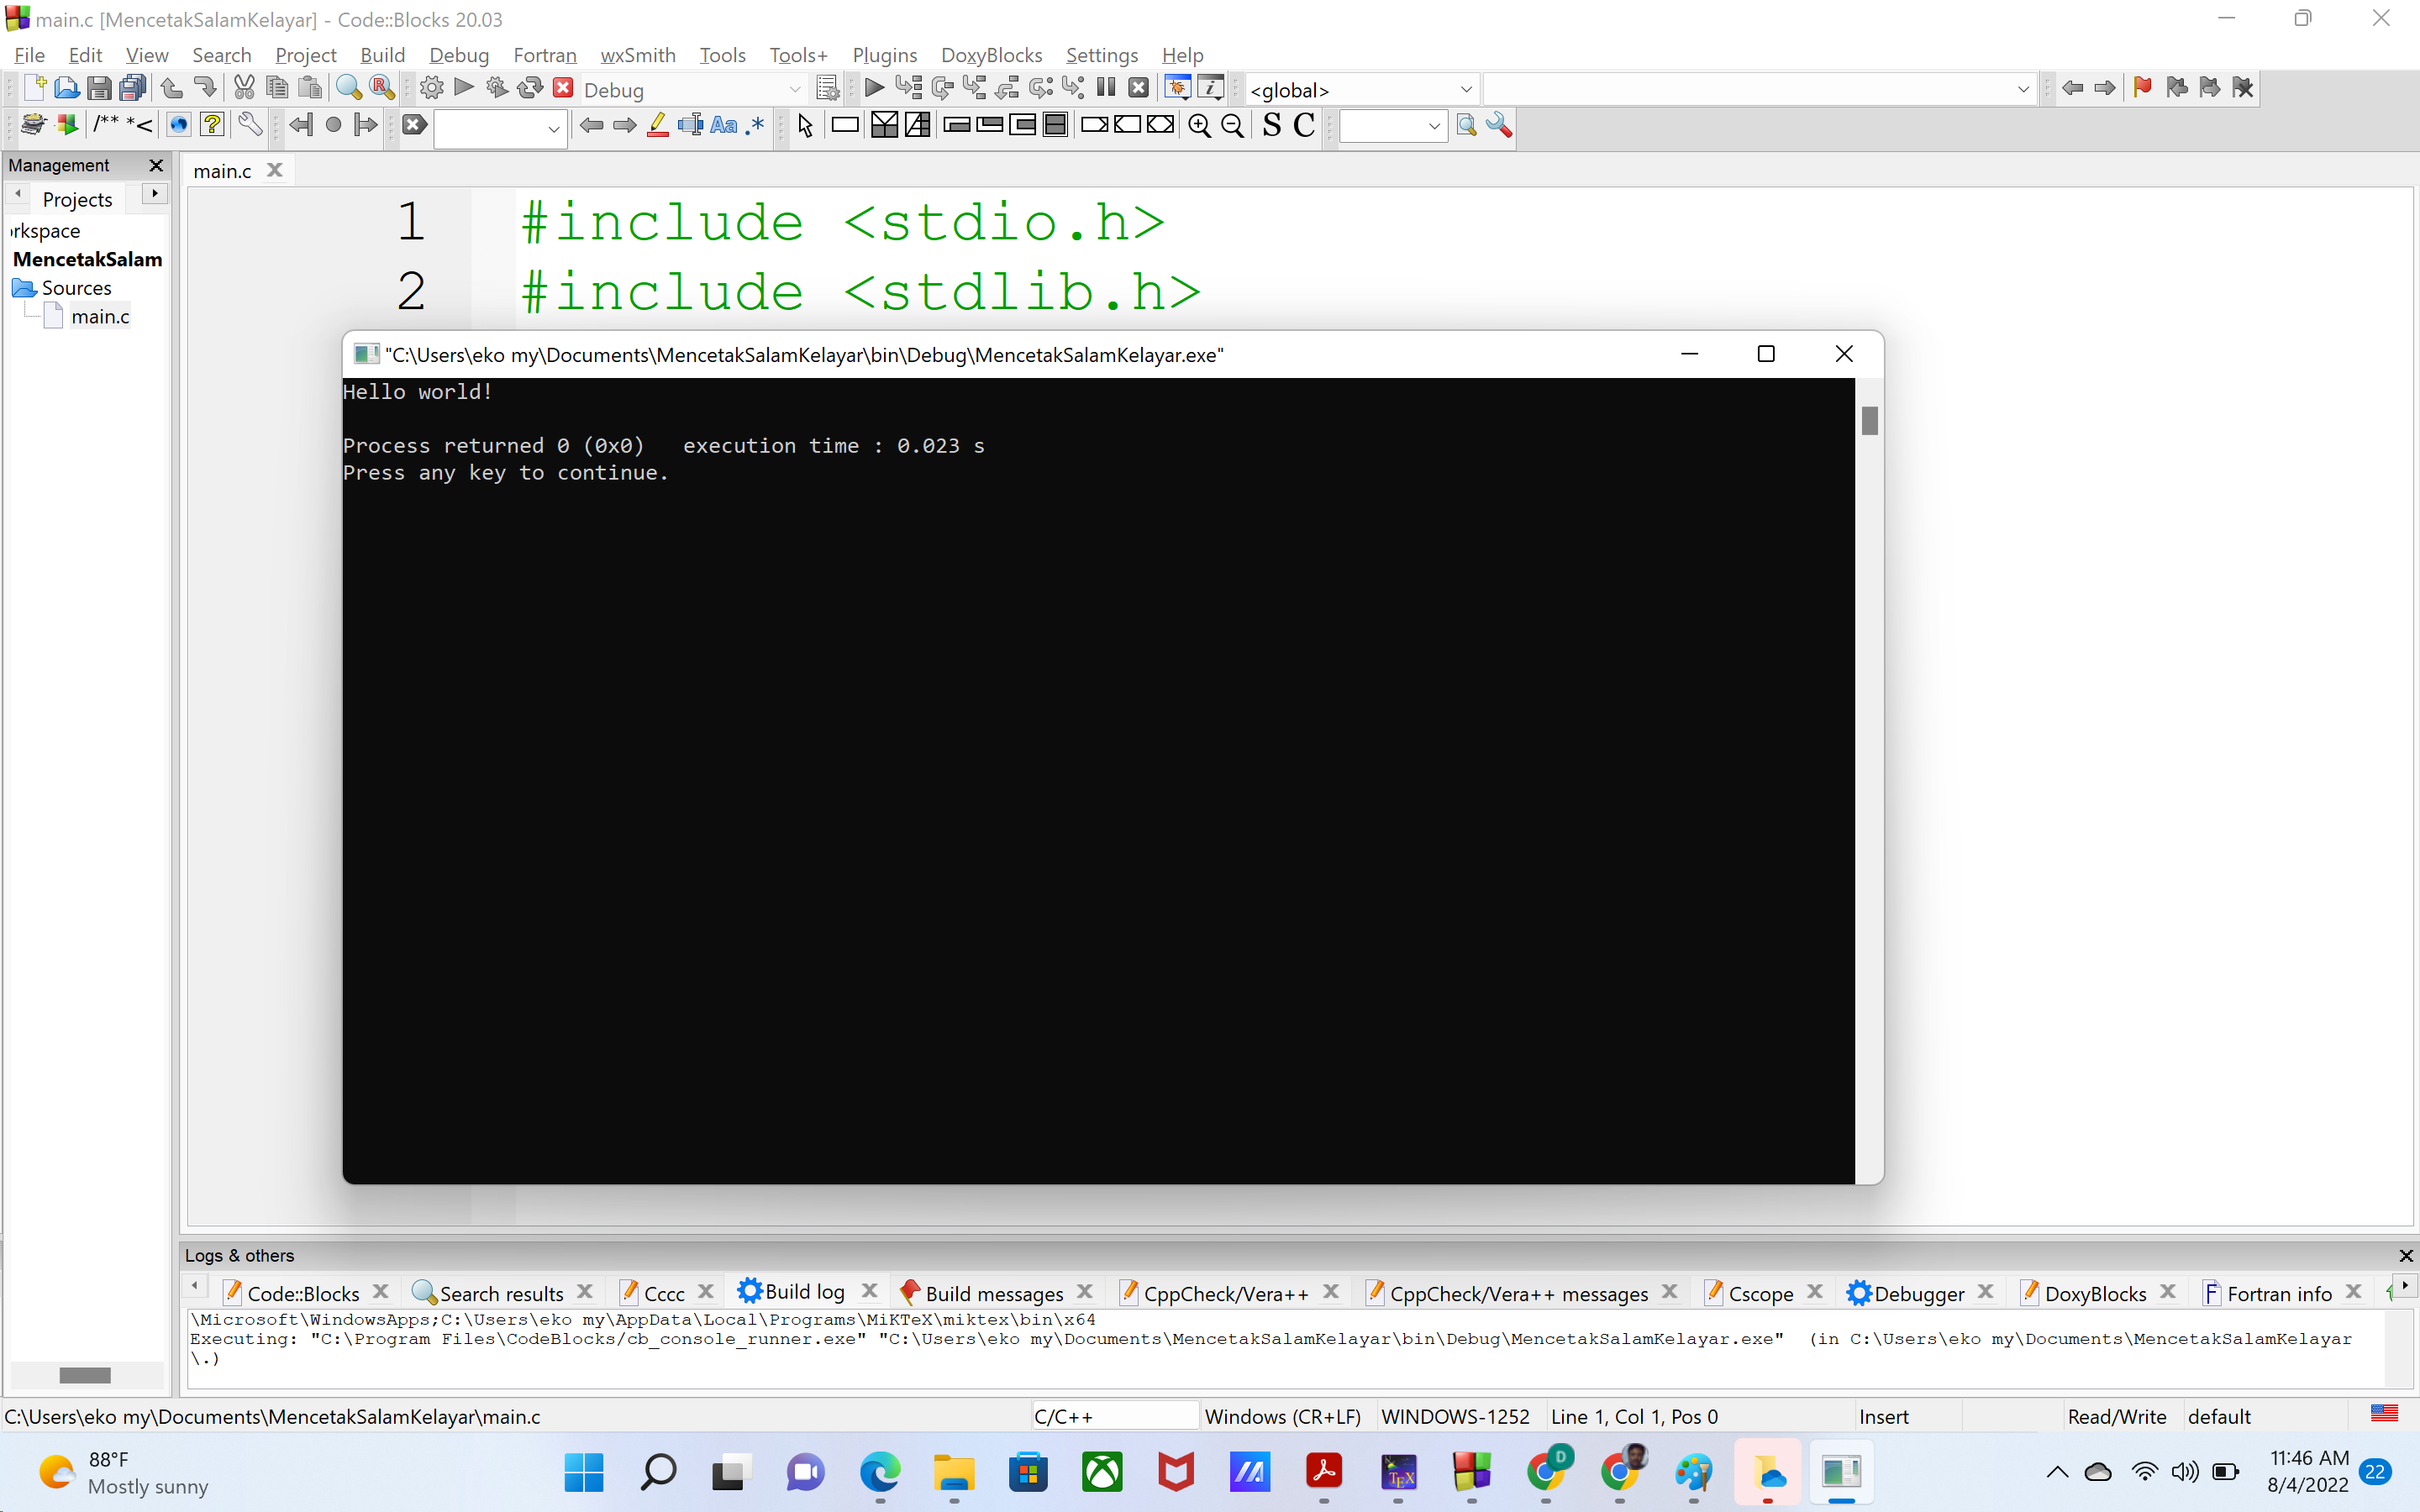
\includegraphics[width=0.7\linewidth]{P1/img/screenshot010.png}
		      \caption{}
		      \label{fig:screenshot010}
	      \end{figure}
\end{enumerate}

\section{Struktur Bahasa C}

\begin{lstlisting}[language=c,caption=Contoh program sederhana dalam bahasa C,label=lst:helloworld,captionpos=t]
	#include <stdio.h>

	int main() {
		printf("Hello World!");
		return 0;
	}
	\end{lstlisting}
Berikut adalah penjelasan kode di atas:
\begin{enumerate}
	\item \verb|#include <stdio.h>|
	merupakan sebuah header dimana kita memasukkan fungsi-fungsi yang ada di dalam file 'stdio.h' yang berisi fungsi input dan output dasar, seperti printf()
	\item int main()
    merupakan fungsi utama. fungsi ini pasti ada di setiap program bahasa C. 
    semua program yang ada di dalam kurung kurawal {} akan dieksekusi ketika program dijalankan.
	\item printf("Hello World!");
    sebuah fungsi untuk mengeluarkan output "Hello Wolrd!".
    bisa diperhatikan di bagian akhir terdapat tanda titik koma ';'. setiap pernyataan (statement) dalam bahasa C selalu diakhiri oleh tanda koma
	\item return 0;
    sebuah pernyataan (statement) yang mengembalikan nilai ke fungsi main(), fungsi akan berakhir ketika dikembalikan.
    program yang ditulis dibawahnya, meskipun masih berada di dalam kurung kurawal akan di abaikan.
\end{enumerate}
Bahasa C mengabaikan spasi (whitespace), sehingga program di atas bisa juga ditulis sebagai:
\begin{lstlisting}[language=c]
	int main(){printf("Hello World!");return 0;}
\end{lstlisting}
tetapi jika ditulis seperti itu akan lebih sulit untuk dibaca.
sehingga lebih baik untuk menulis program dengan spasi dan di baris yang berbeda agar lebih mudah untuk dibaca.

\subsection*{Tugas Pendahuluan 1}
\begin{enumerate}
	\item Dari contoh di atas, apa yang terjadi jika \verb|#include <stdio.h>| dihapus?
  	\item Jika kode ditulis seperti di bawah ini, apa yang terjadi? kenapa hal itu bisa terjadi?
	\begin{lstlisting}[language=c]
	#include <stdio.h>

	int main() {
		return 0;
		printf("Hello World!");
	}
	\end{lstlisting}
\end{enumerate}

\section{Tipe Data}

Dalam bahasa C ada 3 tipe data dasar, yaitu int (integer), float, char (character).

\subsection{integer}

tipe data integer menyimpan data berupa bilangan bulat (tidak ada koma).\\
\begin{center}
	\captionof{table}{Tipe data integer \label{tab:integer}}
	\begin{tabular}{|l|c|l|}
		\hline
		\textbf{Tipe} & \textbf{Ukuran (byte)} & \textbf{Keterangan} \\
		\hline
		int 		& 4 		& tipe dasar integer \\
		short 		& 2 		& menyimpan integer yang lebih kecil \\
		long 		& 4 atau 8 	& menyimpan integer yang lebih besar, tergantung sistem \\
		long long 	& 8 		& bisa menampung angka sangat besar \\
		\hline
	\end{tabular}
\end{center}

\subsection{float}

tipe data float menyimpan data berupa bilangan desimal.
\begin{center}
	\captionof{table}{Tipe data float \label{tab:float}}
	\begin{tabular}{|l|c|l|}
		\hline
		\textbf{Tipe} & \textbf{Ukuran (byte)} & \textbf{Keterangan} \\
		\hline
		float 		& 4 	& tingkat ketelitian yang cukup untuk kebutuhan umum \\
		double 		& 8 	& ketelitian lebih tinggi, cocok untuk penghitungan ilmiah \\
		long double	& 10 	& ketelitian lebih tinggi dari double, tergantung pada compiler \\
		\hline
	\end{tabular}
\end{center}

\subsection{character}

tipe data ini menyimpan data berupa karakter, seperti sebuah huruf 'a', 'b', 'c', atau simbol '@', '\$', '?' dsb.
\begin{center}
	\captionof{table}{Tipe data char \label{tab:char}}
	\begin{tabular}{|l|c|l|}
		\hline
		\textbf{Tipe} & \textbf{Ukuran (byte)} & \textbf{Keterangan} \\
		\hline
		char & 1	& menyimpan kode ASCII. \\
		\hline
	\end{tabular}
\end{center}
ASCII (American Standard Code for Information Interchange) adalah standar kode karakter yang menghubungkan angka (0–127) dengan huruf, angka, tanda baca, dan simbol kontrol.
Dengan ASCII, komputer bisa menyimpan dan memproses teks karena setiap karakter punya kode numerik.

\subsection{Modifier}
Modifier adalah kata kunci tambahan di C yang dipakai untuk mengubah ukuran atau jangkauan nilai suatu tipe data dasar.
Modifier tidak bisa berdiri sendiri, harus digabung dengan tipe data dasar (int, char, dll).
Dalam bahasa C ada 4 modifier yaitu:
\begin{enumerate}
	\item signed \\
	modifier ini ada nilai default untuk int dan char. modifier ini hanya bisa digunakan untuk int dan char.
	dengan modifier ini sebuah tipe data bisa menyimpan nilai negatif dan positif.
    \\ contoh: \texttt{int a;}
	\item unsigned \\
    dengan modifier ini tipe data hanya menyimpan nilai positif.
	\\ contoh: \texttt{unsigned int b;}
    \item short \\
    dengan modifier ini sebuah integer memiliki ukuran lebih kecil, biasanya menjadi 2 bytes.
    \\ contoh: \texttt{short int c;} 
	\item long \\
    dengan modifier ini tipe data akan memiliki ukuran yang lebih besar.
	\\ contoh: \texttt{long int d;}
\end{enumerate}

\subsection*{Tugas Pendahuluan 2}
\begin{enumerate}
	\item Untuk menyimpan angka 2147483648, kita memerlukan tipe data apa? jelaskan!
	\item Jika kita ingin menyimpan nomor HP 12 digit (contoh: 012345678999), tipe data apa yang cocok untuk digunakan? jelaskan alasanmu!
\end{enumerate}


\section{Variabel}

Variabel merupakan sebuah tempat untuk menyimpan data.
Untuk menggunakan variabel, kita perlu mendeklarasikan variabel tersebut terlebih dahulu.
\\ Untuk mendeklarasikan variabel bisa dilakukan dengan cara berikut:
\begin{lstlisting}
	tipe_data nama_variabel.
\end{lstlisting}
\begin{enumerate}[label={}, leftmargin=*]
	\item \verb|tipe_data| adalah tipe data yang ingin kita simpan dalam variabel tersebut (seperti int, float, yang dipelajari di sub bab sebelumnya).
	\item \verb|nama_variabel| adalah nama dari variabelnya.
\end{enumerate}
dalam membuat nama sebuah variabel terdapat aturan yang harus diikuti, yaitu:
\begin{enumerate}
	\item Nama variabel hanya boleh berisi huruf, angka, dan garis bawah (underscore).
	\item Nama variabel harus diawali dengan huruf atau garis bawah, tidak boleh diawali angka.
	\item Spasi tidak diperbolehkan di dalam nama variabel.
	\item Nama variabel tidak boleh berupa kata kunci (keyword) atau reserved word (kata kunci yang sudah ditentukan oleh standar bahasa pemrograman).
	\item Nama variabel harus unik dalam program.
\end{enumerate}
kita juga bisa mendeklarasikan banyak variabel yang memiliki tipe data yang sama dalam 1 baris saja.
contoh: \verb|tipe_data nama1, nama2, nama3;|

\subsection*{inisialisasi variabel}

inisialisasi adalah memberi nilai awal pada variabel saat variabel itu dibuat.
inisialisasi ini penting karena sebuah variabel ketika dideklarasikan akan berisi garbage value(bisa acak).
untuk inisialisasi kita hanya perlu memasukkan nilai ke variabel menggunakan operator "=".
{
\captionsetup[lstlisting]{labelformat=empty, justification=raggedright, singlelinecheck=false} %agar caption tanpa label dan di kiri
\begin{lstlisting}[language=c, caption={syntax}]
	tipe_data nama = nilai_variabel;
\end{lstlisting}
}
untuk mengubah nilai dari sebuah variabel kita bisa menggunakan cara yang sama seperti inisialisasi.
contoh:
\begin{lstlisting}[language=c]
	int a = 5; // inisialisasi variabel a bernilai 5
	a = 12; // nilai a berubah menjadi 12
\end{lstlisting}

\subsection*{Tugas Pendahuluan 3}
\begin{enumerate}
	\item perhatikan kode berikut:
	\begin{lstlisting}[language=c]
	int 2angka = 10;
	float tinggi-badan = 170,5;
	char nama lengkap = ' B ';
\end{lstlisting}
	kode di atas berisi deklarasi beberapa variabel.
	Sebutkan semua kesalahan yang ada pada kode tersebut dan jelaskan alasannya!
	Berikan contoh penulisan kode yang benar!
	\item perhatikan kode berikut:
	\begin{lstlisting}[language=c]
	const int a = 5;
	int b = 2;
	a++;
	b++;
\end{lstlisting}
	kode di atas terdapat sebuah error. Kenapa error tersebut terjadi? bagaimana cara memeperbaikinya?
\end{enumerate}

\section{Komentar}
komentar adalah sebuah baris atau bagian dari program yang diabaikan ketika dijalankan.
Komentar dapat digunakan untuk menjelaskan kode, dan membuatnya lebih mudah dibaca.
Komentar juga bisa digunakan untuk mencegah eksekusi kode saat melakukan pengujian.
\\ untuk menulis sebuah komentar dalam bahasa C, kita menggunakan double slash "//", semua hal yang ditulis setelah "//" dalam satu baris akan menjadi komentar.
contoh :
\begin{lstlisting}[language=c]
	//ini komentar
  	printf("halo dunia"); //ini juga komentar
	// printf("Kode di baris ini tidak akan berjalan");
\end{lstlisting}
komentar juga bisa ditulis dalam banyak baris dengan menggunakan "/*" dan "*/".
semua hal yang ditulis diantara "/*" dan "*/" akan menjadi komentar.
contoh:
\begin{lstlisting}[language=c]
/*
Contoh komentar
dengan banyak baris
*/
\end{lstlisting}

\subsection*{Tugas Pendahuluan 4}
\begin{enumerate}
	\item Perhatikan kode berikut:
	\begin{lstlisting}
	/*
		Ini adalah komentar
		/*
		komentar ini ada di dalam komentar
		*/
	*/
\end{lstlisting}
	Apakah penulisan komentar di atas benar? jika tidak, kenapa penulisannya salah?
	\item Untuk membuat komentar dengan banyak baris, kita bisa menggunakan tanda "/*" dan "*/".
	Apa yang terjadi jika hanya menggunakan tanda "/*" saja?
\end{enumerate}

\section{Operator}

Operator merupakan simbol yang merepresentasikan sebuah operasi yang dilakukan oleh sebuah atau beberapa nilai dan variabel.
nilai dan variabel yang digunakan dalam sebuah operasi disebut dengan operand.
\\ Dalam bahasa C, operator dibedakan menjadi 6 jenis berdasarkan fungsinya, yaitu:

\subsection{Operator Aritmatika}

digunakan untuk melakukan operasi aritmatika.
\begin{center}
	\captionof{table}{Operator Aritmatika\label{tab:aritmatika}}
	\begin{tabular}{|c|c|p{6cm}|c|}
		\hline
		\multicolumn{1}{|c|}{\textbf{Simbol}} &
		\multicolumn{1}{c|}{\textbf{Nama Operator}} &
		\multicolumn{1}{c|}{\textbf{Deskripsi}} &
		\multicolumn{1}{c|}{\textbf{Sintaks}} \\ \hline
		+   & Penjumlahan          & Menambahkan dua buah angka & a + b \\ \hline
		-   & Pengurangan          & Mengurangi angka pertama dengan angka kedua & a - b \\ \hline
		*   & Perkalian            & Mengalikan kedua angka & a * b \\ \hline
		/   & Pembagian            & Membagi angka pertama dengan angka kedua & a / b \\ \hline
		\%  & Modulus              & Menghasilkan sisa dari pembagian angka pertama dengan angka kedua & a \% b \\ \hline
		+   & Plus (unary)         & Menandakan sebuah angka merupakan bilangan positif & +a \\ \hline
		-   & Minus (unary)        & Menandakan sebuah angka merupakan bilangan negatif & -a \\ \hline
		++  & Increment            & Menambah nilai sebuah angka sebanyak 1 & a++ \\ \hline
		--  & Decrement            & Mengurangi nilai sebuah angka sebanyak 1 & a-- \\ \hline
	\end{tabular}
\end{center}


\subsection{Operator Relasional/Pembanding}

Digunakan untuk membandingkan dua operand.
Semua operator pembanding akan menghasilkan nilai true atau false sebagai hasil dari perbandingannya.
\begin{center}
	\captionof{table}{Operator Pembanding\label{tab:relasional}}
	\begin{tabular}{|c|p{3cm}|p{6cm}|c|}
		\hline
		\multicolumn{1}{|c|}{\textbf{Simbol}} &
		\multicolumn{1}{c|}{\textbf{Nama Operator}} &
		\multicolumn{1}{c|}{\textbf{Deskripsi}} &
		\multicolumn{1}{c|}{\textbf{Sintaks}} \\ \hline
		<   & Lebih kecil                & Bernilai benar jika operand kiri lebih kecil dari operand kanan & a < b \\ \hline
		>   & Lebih besar                & Bernilai benar jika operand kiri lebih besar dari operand kanan & a > b \\ \hline
		<=  & Lebih kecil atau sama dengan & Bernilai benar jika operand kiri lebih kecil atau sama dengan operand kanan & a <= b \\ \hline
		>=  & Lebih besar atau sama dengan & Bernilai benar jika operand kiri lebih besar atau sama dengan operand kanan & a >= b \\ \hline
		==  & Sama dengan                & Bernilai benar jika kedua operand bernilai sama & a == b \\ \hline
		!=  & Tidak sama dengan          & Bernilai benar jika kedua operand tidak sama & a != b \\ \hline
	\end{tabular}
\end{center}

\subsection{Operator Logika}

digunakan untuk menentukan logika antara kedua operand.
\begin{center}
	\captionof{table}{Operator Logika \label{tab:logic}}
	\begin{tabular}{|c|c|p{7cm}|c|}
		\hline
		\multicolumn{1}{|c|}{\textbf{Simbol}} &
		\multicolumn{1}{c|}{\textbf{Nama Operator}} &
		\multicolumn{1}{c|}{\textbf{Deskripsi}} &
		\multicolumn{1}{c|}{\textbf{Sintaks}} \\ \hline
		\texttt{\&\&} & Logika AND & Bernilai benar jika kedua operand bernilai benar & \texttt{a \&\& b} \\ \hline
		\texttt{||}   & Logika OR  & Bernilai benar jika salah satu atau kedua operand bernilai benar & \texttt{a || b} \\ \hline
		\texttt{!}    & Logika NOT & Bernilai benar jika operand bernilai salah & \texttt{!a} \\ \hline
	\end{tabular}
\end{center}

\subsection{Operator Bitwise}

Digunakan untuk melakukan operasi pada tingkat bit.
Operand akan diubah menjadi bilangan biner terlebih dahulu lalu baru dilakukan operasi pada operand tersebut.
\begin{center}
	\captionof{table}{Operator Bitwise \label{tab:bitwise}}
	\begin{tabular}{|c|l|p{8cm}|c|}
		\hline
		\multicolumn{1}{|c|}{\textbf{Simbol}} &
		\multicolumn{1}{c|}{\textbf{Nama Operator}} &
		\multicolumn{1}{c|}{\textbf{Deskripsi}} &
		\multicolumn{1}{c|}{\textbf{Sintaks}} \\ \hline
		\texttt{\&}  & Bitwise AND              & Melakukan operasi AND per bit dan mengembalikan hasilnya & \texttt{a \& b} \\ \hline
		\texttt{|}   & Bitwise OR               & Melakukan operasi OR per bit dan mengembalikan hasilnya & \texttt{a | b} \\ \hline
		\texttt{\^}  & Bitwise XOR              & Melakukan operasi XOR per bit dan mengembalikan hasilnya & \texttt{a \^ b} \\ \hline
		\texttt{\~}  & Bitwise NOT (Komplemen)  & Membalik semua bit (0 jadi 1, 1 jadi 0) & \texttt{\~a} \\ \hline
		\texttt{<<}  & Bitwise Left Shift       & Menggeser bit ke kiri sebanyak n posisi; ekuivalen dengan perkalian 2 tiap geseran & \texttt{a << b} \\ \hline
		\texttt{>>}  & Bitwise Right Shift      & Menggeser bit ke kanan sebanyak n posisi; ekuivalen dengan pembagian 2 tiap geseran & \texttt{a >> b} \\ \hline
	\end{tabular}
\end{center}

\subsection{Operator Penugasan (Assignment)}

Digunakan untuk emmberi nilai ke variabel.
\begin{center}
	\captionof{table}{Operator Assignment \label{tab:assignment}}
	\begin{tabular}{|c|l|p{8cm}|c|}
		\hline
		\multicolumn{1}{|c|}{\textbf{Simbol}} &
		\multicolumn{1}{c|}{\textbf{Nama Operator}} &
		\multicolumn{1}{c|}{\textbf{Deskripsi}} &
		\multicolumn{1}{c|}{\textbf{Sintaks}} \\ \hline
		=   & Assignment Sederhana & Memberikan nilai dari operand kanan ke operand kiri. & a = b \\ \hline
		+=  & Tambah dan Assign & Menjumlahkan operand kanan dengan operand kiri, lalu hasilnya disimpan ke operand kiri. & a += b \\ \hline
		-=  & Kurang dan Assign & Mengurangi operand kiri dengan operand kanan, lalu hasilnya disimpan ke operand kiri. & a -= b \\ \hline
		*=  & Kali dan Assign & Mengalikan operand kiri dengan operand kanan, lalu hasilnya disimpan ke operand kiri. & a *= b \\ \hline
		/=  & Bagi dan Assign & Membagi operand kiri dengan operand kanan, lalu hasilnya disimpan ke operand kiri. & a /= b \\ \hline
		\%=  & Modulus dan Assign & Mengambil sisa hasil bagi operand kiri dengan operand kanan, lalu hasilnya disimpan ke operand kiri. & a \%= b \\ \hline
		\&=  & AND Bitwise dan Assign & Melakukan operasi bitwise AND, lalu hasilnya disimpan ke operand kiri. & a \&= b \\ \hline
		|=  & OR Bitwise dan Assign & Melakukan operasi bitwise OR, lalu hasilnya disimpan ke operand kiri. & a |= b \\ \hline
		\verb|^=|  & XOR Bitwise dan Assign & Melakukan operasi bitwise XOR, lalu hasilnya disimpan ke operand kiri. & a \verb|^=| b \\ \hline
		>>= & Rightshift dan Assign & Menggeser bit operand kiri ke kanan, lalu hasilnya disimpan ke operand kiri. & a >>= b \\ \hline
		<<= & Leftshift dan Assign & Menggeser bit operand kiri ke kiri, lalu hasilnya disimpan ke operand kiri. & a <<= b \\ \hline
	\end{tabular}
\end{center}

\subsection{Operator Lainnya}

Selain operator di atas, dalam bahasa C terdapat operator lain yang digunakan untuk tugas spesifik.
Kita akan mendalami operator-operator ini pada modul berikutnya.
\begin{enumerate}
	\item \textbf{operator kondisional (?:)} \\
	ini adalah satu-satunya operator ternary (operator yang memiliki 3 buah operand) dalam bahasa C.
	digunakan untuk memeriksa suatu kondisi (pengganti if). \\
	contoh : \verb|kondisi ? hasil_jika_benar : hasil_jika_salah|
	\item \textbf{operator dot (.) dan arrow (->)} \\
	digunakan untuk mengakses member dalam struct \\
	\verb|structure_variable . member;| \\
	\verb|structure_pointer -> member;|
	\item \textbf{operator addressof (\&) dan Dereference (*)} \\
	operator '\&' mengembalikan nilai alamat dari sebuah variabel. \\
	contoh: \verb|&var| merupakan alamat dari variabel var \\
	operator '*' merupakan pointer kesebuah variabel. \\
	contoh: \verb|*var| merupakan pointer ke variabel var
\end{enumerate}

\subsection*{Tugas Pendahuluan 5}
\begin{enumerate}
	\item perhatikan kode berikut:
	\begin{lstlisting}[language=c]
	int a = 5;
	int b = 2;
	a += b += 3;
\end{lstlisting}
    Setelah kode tersebut dijalankan, berapa nilai a dan b? jelaskan langkah-langkahnya! jika ada error, jelaskan kenapa dan perbaiki kodenya!
	\item perhatikan kode berikut:
	\begin{lstlisting}[language=c]
	int m = 10, n = 3;
	int hasil = m / n;
\end{lstlisting}
    Setelah kode tersebut dijalankan, berapa nilai hasil? jelaskan langkah-langkahnya! jika ada error, jelaskan kenapa dan perbaiki kodenya!
  	\item perhatikan kode berikut:
  	\begin{lstlisting}[language=c]
	int m = 10, n = 3;
	int hasil = m / n += 2;
\end{lstlisting}
    Setelah kode tersebut dijalankan, berapa nilai hasil? jelaskan langkah-langkahnya! jika ada error, jelaskan kenapa dan perbaiki kodenya!
\end{enumerate}

\section{Output}

Dalam sub-bab syntax kita sudah mempelajari terkait printf("Hello World!");, fungsi printf() ini merupakan fungsi yang digunakan untuk mengeluarkan sebuah output ke terminal.
  Terminal adalah aplikasi untuk menjalankan perintah teks agar bisa berinteraksi dengan komputer, misalnya membuka folder, mengelola file, atau menjalankan program.
  fungsi printf() bisa kita tulis dengan Syntax
{
\captionsetup[lstlisting]{labelformat=empty, justification=raggedright, singlelinecheck=false} %agar caption tanpa label dan di kiri
\begin{lstlisting}[language=c, caption={syntax}]
	printf("format_string", variables/values);
\end{lstlisting}
}
\begin{enumerate}[label={}, leftmargin=*]
	\item formatted\_string : sebuah string yang akan dikeluarkan sebagai output, didalamnya bisa memiliki 'format specifier'
	\item variables/values : sebuah argument yang akan menggantikan format specifier yang ada dalam formatted\_string.
\end{enumerate}

\subsection{Format Specifier}
Format specifier adalah tanda khusus yang dipakai di dalam fungsi input/output (printf, scanf) untuk memberi tahu compiler tipe data apa yang akan ditampilkan atau dibaca.
Macam-macam format specifier:
\begin{center}
	\captionof{table}{Format Specifier dalam C \label{tab:format-specifier}}
	\begin{tabular}{|c|p{7cm}|c|}
		\hline
		\textbf{Specifier} & \textbf{Keterangan} & \textbf{Contoh Output} \\ \hline
		\%d   & integer (bilangan bulat) & 10 \\ \hline
		\%f   & float/double (bilangan pecahan) & 3.14 \\ \hline
		\%.2f  & 2 angka di belakang koma (angka 2 bisa diganti untuk mengatur jumlah angka di belakang koma) & 3.14 \\ \hline
		\%c   & char (karakter) & A \\ \hline
		\%s   & string (array of char) & Hello \\ \hline
		\%u   & unsigned integer & 25 \\ \hline
		\%o   & oktal & 017 \\ \hline
		\%x   & heksadesimal (huruf kecil) & 1a \\ \hline
		\%X   & heksadesimal (huruf besar) & 1A \\ \hline
		\%p   & alamat pointer & 0x7ffee \\ \hline
		\%\%  & tanda persen & \% \\ \hline
	\end{tabular}
\end{center}
Contoh:
\begin{lstlisting}[language=c]
#include <stdio.h>

int main() {
	int nrp = 5024991000;
	float ipk = 3.99;
	char grade = 'A';

	printf("Umur   : %d\n", nrp);	  // print output bilangan bulat
	printf("IPK    : %.2f\n", ipk);   // print output bilanghan desimal dengan 2 angka di belakang koma
	printf("Grade  : %c\n", grade);	  // print output karakter

	return 0;
}
\end{lstlisting}

\subsection{Escape Sequence}

Escape sequence adalah karakter khusus yang diawali dengan backslash (\textbackslash) dan dipakai di dalam string untuk mengontrol tampilan output.
\begin{center}
	\captionof{table}{Escape Sequence dalam C \label{tab:escape}}
	\begin{tabular}{|c|l|p{7.5cm}|}
		\hline
		\multicolumn{1}{|c|}{\textbf{Escape Sequence}} &
		\multicolumn{1}{c|}{\textbf{Nama}} &
		\multicolumn{1}{c|}{\textbf{Arti / Fungsi}} \\ \hline
		\textbackslash n   & Newline & Pindah ke baris baru \\ \hline
		\textbackslash t   & Horizontal Tab & Memberi jarak tab \\ \hline
		\textbackslash\textbackslash & Backslash & Menampilkan karakter backslash \textbackslash \\ \hline
		\textbackslash"   & Double Quote & Menampilkan tanda kutip ganda " \\ \hline
		\textbackslash'   & Single Quote & Menampilkan tanda kutip tunggal ' \\ \hline
		\textbackslash r   & Carriage Return & Kembali ke awal baris \\ \hline
		\textbackslash b   & Backspace & Menghapus 1 karakter sebelumnya \\ \hline
		\textbackslash f   & Form Feed & Pindah halaman (jarang dipakai) \\ \hline
		\textbackslash a   & Bell / Alert & Bunyi beep (tergantung sistem) \\ \hline
		\textbackslash 0   & Null Character & Penutup string di C \\ \hline
	\end{tabular}
\end{center}
Contoh:
\begin{lstlisting}[language=c]
#include <stdio.h>

int main() {
	printf("Hello\nWorld\n");         // baris baru
	printf("Nama:\tB300\n");          // tab
	printf("Kata hari ini: \"Bernafas\"\n"); // kutip ganda
	printf("C:\\Users\\Public\n");   // menampilkan path dengan \
	return 0;
}
\end{lstlisting}

\subsection*{Tugas Pendahuluan 6}
\begin{enumerate}
	\item Perhatikan kode berikut:
	\begin{lstlisting}[language=c]
	int main() {
		float a = 3.14;

		printf("%d", a);

		return 0;
	}
\end{lstlisting}
    Berapa nilai output yang ditampilkan? kenapa outputnya nilai itu? jika kita ingin outputnya itu "3.14", perubahan apa yang perlu dilakukan?
  	\item Buatlah sebuah program sederhana yang mengeluarkan output \verb|\'\'\'\'\'| !
\end{enumerate}

\section{Input}

dalam bahasa C, fungsi input yang sering digunakan adalah scanf().
scanf() bisa ditulis seperti berikut:
{
\captionsetup[lstlisting]{labelformat=empty, justification=raggedright, singlelinecheck=false} %agar caption tanpa label dan di kiri
\begin{lstlisting}[language=c, caption={syntax}]
	scanf("format", &var1, &var2, ...);
\end{lstlisting}
}
\begin{enumerate}[label={}, leftmargin=*]
	\item \verb|format|: sama seperti printf, ini berisi string dan juga format specifier.
\end{enumerate}
untuk variabel wajib menggunakan operator '\&' untuk mendapatkan alamat dari variabel.
\\ Contoh:
\begin{lstlisting}[language=c]
#include <stdio.h>

int main() {
	int umur;
	float ipk;
	char grade;

	// Input integer
	scanf("%d", &umur);

	// Input float
	scanf("%f", &ipk);

	// Input karakter
	scanf(" %c", &grade);

	// Output hasil input
	printf("\n=== Data ===\n");
	printf("Umur  : %d\n", umur);
	printf("IPK   : %.2f\n", ipk);
	printf("Grade : %c\n", grade);

	return 0;
}
\end{lstlisting}
\begin{verbatim}
	INPUT :
	21
	3.85
	A

	OUTPUT :
	=== Data ===
	Umur  : 21
	IPK   : 3.85
	Grade : A
\end{verbatim}
Dalam satu scanf() kita bisa mendapatkan banyak input untuk beberapa variabel.
Sehingga bagian scanf pada kode di atas bisa ditulis menjadi:
\begin{lstlisting}[language=c]
	// Input untuk ketiga variabel
	scanf("%d %f %c", &nrp, &ipk, &grade);
\end{lstlisting}

\subsection*{Tugas Pendahuluan 7}
\begin{enumerate}
	\item pada \verb|scanf("%d", &angka);| program meminta input integer untuk dimasukkan ke variabel angka.
     apa yang terjadi jika kita tulis \verb|scanf("%d", angka);| ? kenapa penulisan operator '\&' penting di scanf() ?
  	\item buatlah program sederhana yang menerima input dua angka integer lalu menampilkan hasil pembagian angka pertama dengan angka kedua di layar!
\end{enumerate}


% \section{Tujuan}
\begin{itemize}[label=$\bullet$, itemsep=-1pt, leftmargin=*]
	\item Mahasiswa mengenal dan mampu menggunakan ekspresi-ekspresi logika dan perbandingan pada bahasa pemrograman C
	\item Mahasiswa mengenal dan mampu menggunakan syntax-syntax percabangan pada bahasa pemrograman C
	\item Mahasiswa dapat mengenal dan menggunakan perulangan while pada bahasa C
	      % \item Students are able to use while-loop on C
	\item Mahasiswa dapat mengenal dan menggunakan perulangan do-while pada bahasa C
	      % \item Students are able to use do-while loop on C
	\item Mahasiswa dapat mengenal dan menggunakan perulangan for pada bahasa C
	      % \item Students are able to use for loop on C
	\item Mahasiswa dapat mengenal dan menggunakan  array dimensi satu maupun multidimensi.
	      % \item Students are able to use one dimensional or multidimensional array
	\item Mahasiswa mampu memanfaatkan perulangan untuk mengolah data pada array.
	      % \item Students are able to use loops to process data on arrays
	\item Mahasiswa  dapat mengenal dan menggunakan  string.
\end{itemize}
\section{Ekspresi Logika dan Perbandingan}
\subsection{Ekspresi Perbandingan}
Berikut adalah operator-operator yang digunakan pada suatu ekspresi perbandingan
% The following are the operators used in comparison expressions.
\begin{center}
	\captionof{table}{Operator Perbandingan \label{tab:operatorcomp}}
	\begin{tabular}{|c|l|c|}
		\hline
		Operator        & Nama                    & \multicolumn{1}{l|}{Contoh Ekspres} \\ \hline
		==              & Sama Dengan             & x == y                              \\ \hline
		!=              & Tidak Sama Dengan       & x != y                              \\ \hline
		\textgreater{}  & Lebih Dari              & x \textgreater y                    \\ \hline
		\textless{}     & Kurang Dari             & x \textless y                       \\ \hline
		\textgreater{}= & Lebih Dari Sama Dengan  & x \textgreater{}= y                 \\ \hline
		\textless{}=    & Kurang Dari Sama Dengan & x \textless{}= y                    \\ \hline
	\end{tabular}
\end{center}

Suatu ekspresi perbandingan akan mengembalikan nilai berupa \verb|true| atau \verb|false| yang ditandakan dengan nilai 0 atau 1.
% A Comparison Expression will return boolean value \verb|true| or \verb|false| which is also represented with the value 1 or 0.
Sebagai contoh:
As example:
\begin{verbatim}
    printf("%d",0>1); // Akan Mencetak 0 ke layar
    printf("%d",0<1); // Akan Mencetak 1 ke layar 
\end{verbatim}

\subsection{Ekspresi Logika}
Berikut adalah operator-operator logika yang digunakan pada suatu ekspresi logika
% The following are the logical operators used on a Logical Expression
\begin{center}
	\captionof{table}{Ekspresi Logika \label{tab:operatorlogic}}
	\begin{tabular}{|c|l|c|}
		\hline
		Operator & \multicolumn{1}{c|}{Nama} & Contoh Ekspresi        \\ \hline
		$\&\&$   & AND                       & $x<5\; \&\& \;x<10$    \\ \hline
		$||$     & OR                        & $x < 5\; ||\; x < 4  $ \\ \hline
		$!$      & NOT                       & $!(x <5 \&\& x < 10) $ \\ \hline
	\end{tabular}
\end{center}
Sama seperti ekspresi perbandingan, ekspresi logika akan mengembalikan nilai berupa true atau false
% Like comparison expression, logical expression will return boolean values.

\section{Percabangan}
\subsection{Pernyataan If}
% \verb*|if| statement is used to decide which block of code to be executed if the condition is true.
\verb*|if| digunakan untuk menentukan blok kode C yang dijalankan apabila ekspresi kondisi bernilai benar (TRUE),
\begin{verbatim}
// Block of code before if
if (Condition) 
{
 // Blok kode yang akan dieksekusi jika kondisinya benar(True).
}
// Blok kode setelah if
\end{verbatim}
Sebagai contoh, perhatikan program berikut
% As example, look at the following code 
\begin{lstlisting}[language=c,caption =Contoh Pernyataan If,label=lst:ifexample01]
	include <stdio.h>
	
	int main()
	{
		//Deklarasi variabel 
		int uangSaya,hargaRoti;
		uangSaya = 5000;
		hargaRoti = 10000;
		
		if (uangSaya>=hargaRoti)
		{
		    printf("saya bisa beli roti\n");
		}
		printf("hehe");
		return 0;
	}
\end{lstlisting}
Keluaran program ini
\begin{verbatim}
    hehe
\end{verbatim}
% If line 7 changed to \verb|uangSaya=10000|, the outputs of the program would be
Jika baris ke 7 diganti dengan \verb|uangSaya=10000| maka output dari program ini akan menjadi
\begin{verbatim}
    saya bisa beli roti
    hehe
\end{verbatim}

\subsection{Pernyataan If-else}
Pernyataan else digunakan untuk menentukan blok kode yang di jalankan apabila kondisi salah.
% Else statement is used to decide the block of code to be executed if the condition is false.
\begin{verbatim}
// Blok kode sebelum if
if (Condition) 
{
	// Blok kode yang akan dieksekusi jika kondisinya benar
} else
{
	// Blok kode yang akan dieksekusi jika kondisinya salah
}
// Blok kode setelah pernyataan if-else
\end{verbatim}
Berikut contoh penggunaan if-else
% The following is an example of using if-else statement:
\begin{lstlisting}[language=c,caption = if-else example,label=lst:ifelseexample01]
	include <stdio.h>
	
	int main()
	{
		//Deklarasi variabel 
		int uangSaya,hargaRoti;
		uangSaya = 5000;
		hargaRoti = 10000;
		
		if (uangSaya>=hargaRoti)
		{
		    printf("saya bisa beli roti\n");
		}
		else
		{
	        printf("saya tidak bisa beli roti\n");	
		}
		printf("hehe");
		return 0;
	}
\end{lstlisting}
Keluaran program adalah sebagai berikut
\begin{verbatim}
    saya tidak bisa beli roti
    hehe
\end{verbatim}
Jika baris ke 7 diganti dengan \verb|uangSaya=10000| maka output dari program ini akan menjadi
% If line 7 changed to \verb|uangSaya=10000|, the outputs of the program would be
\begin{verbatim}
    saya bisa beli roti
    hehe
\end{verbatim}

\subsection{Pernyataan if-else if}
Statement \verb|else if| digunakan untuk menjalankan blok kode apabila kondisi statement \verb|if| atau \verb|else if| sebelumnya bernilai salah.
% The \verb|else if| statement is used to run a block of code when the condition in \verb|if| or the previous \verb|else if| is false.
\begin{verbatim}
	// blok kode sebelum if
    if (Condition1)
    {
	  /* blok kode yang akan dieksekusi jika Kondisi 1
	  adalah benar*/
    }
    else if (Condition2)
    {
	  /* blok kode yang akan dieksekusi jika Kondisi 1 salah
	  dan Kondisi 2 benar */
    }
    else if (Condition3)
    {
	  /* Blok kode yang akan dieksekusi kapan
	  Kondisi 1 dan Kondisi 2 salah dan
	  Kondisi 3 benar*/
    }
    ...
    else if (ConditionN)
    {
	  /*Blok kode yang akan dieksekusi kapan
	  Kondisi 1 hingga KondisiN-1 salah dan
	  Kondisi N benar*/
    }
    else
    {
	  /* Blok kode yang akan dieksekusi kapan
	  Kondisi 1 hingga Kondisi N salah*/
    }
	// Blok kode setelah if
\end{verbatim}
Berikut contoh penggunaan if-else if
\begin{lstlisting}[language=c,caption = Contoh if-else if,label=lst:ifelseifexample01]
	include <stdio.h>
	
	int main()
	{
		//Deklarasi variabel 
		int uangSaya,hargaRoti;
		uangSaya = 5000;
		hargaRoti = 10000;
		
		if (uangSaya>hargaRoti)
		{
		    printf("saya bisa beli roti\n");
		}
		else if(uangSaya==hargaRoti)
		{
		    printf("saya bisa beli roti tapi uang saya akan langsung habis\n");
		}
		else
		{
	        printf("saya tidak bisa beli roti\n");	
		}
		printf("hehe");
		return 0;
	}
\end{lstlisting}
Output dari program ini adalah
\begin{verbatim}
    saya tidak bisa beli roti
    hehe
\end{verbatim}
Jika baris ke 7 diganti dengan \verb|uangSaya=10000| maka output dari program ini akan menjadi
% If line 7 changed to \verb|uangSaya=10000|, the output of the program would be
\begin{verbatim}
    saya bisa beli roti tapi uang saya akan langsung habis
    hehe
\end{verbatim}
Jika baris ke 7 diganti dengan \verb|uangSaya=12000| maka output dari program ini akan menjadi
% If line 7 changed to \verb|uangSaya=12000|, the output of the program would be
\begin{verbatim}
    saya bisa beli roti
    hehe
\end{verbatim}

\subsection{Nested if}
Nested if merupakan konsep di mana di dalam suatu blok if terdapat statement if.
% Nested if is when there is a conditional statements within a block of code inside the conditional statement
\begin{verbatim}
// Blok kode sebelum if
if (Condition1) 
{
    if (Condition2)
    {
        // lakukan sesuatu
    }
    else
    {
        // lakukan sesuatu yang lain
    }
} 
else
{
    // melakukan sesuatu yang lain
}
\end{verbatim}

Berikut contoh penggunaan nested if
% Below is an example of using nested if

\begin{lstlisting}[language=c,caption = Contoh nested if,label=lst:nestedifexample01]
	include <stdio.h>
	
	int main()
	{
		// Declare the variables
		int myMoney,breadPrice,friendsMoney;
		myMoney = 5000;
		breadPrice = 10000;
		friendsMoney = 42069;
		
		
		if (myMoney>breadPrice)
		{
		    printf("I can buy bread\n");
		}
		else if(myMoney==breadPrice)
		{
		    printf("I can buy bread but I will ran out of money\n");
		}
		else
		{
		    if(friendsMoney+myMoney >= breadPrice)
		    {
		        printf("I can buy bread if I borrow my friend money\n"); 
		    }
		    else
		    {
	            printf("I can't buy bread\n");	
		    }
		}
		printf("hehe");
		return 0;
	}
\end{lstlisting}


\subsection{Tugas Pendahuluan}
\begin{enumerate}
	\item Buatlah program yang menerima input 3 buah bilangan bulat A, B, dan C. Outputkanlah 3 bilangan bulat itu ke layar dengan urutan paling kecil ke paling besar. Lakukanlah ini dengan menggunakan statement if, if else, if else if, atau nested if.
	      %\item Try to make a program that receives 3 integer input A, B, and C. Then outputs those 3 integers to the screen sorted from smallest to largest. Do this only using conditional statements.	
\end{enumerate}

\section{Perulangan}
\subsection{Perulangan while}
Perulangan while akan menjalankan blok kode yang berada di dalamnya selama kondisi perulangan masih bernilai benar.
% While loop will run the code block within it repeatedly as long as the loop condition is true


\begin{figure}[H]
	\centering
	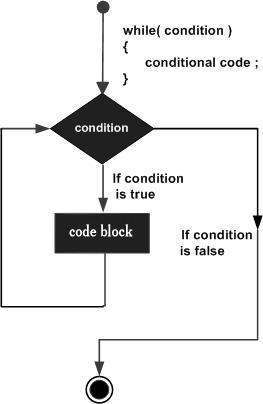
\includegraphics[width=0.4\linewidth]{P2/img/whileloop.png}
	\caption{Flow chart perulangan while}
	\label{fig:whileloop}
\end{figure}

Syntaxnya pada bahasa C adalah sebagai berikut:
% Its syntax in C programming language is as follows
\begin{verbatim}
    while(Condition)
    {
        // Blok kode yang akan diulang
    }
\end{verbatim}

Sebagai contoh, perhatikan kode berikut
% As an example, look at the following code
\begin{lstlisting}[language=c,caption = Contoh Penggunaan while,label=lst:whileexample01]
int main()
{
	int uangSaya,hargaRoti;
	uangSaya = 10000;
	hargaRoti = 2000;
	while(uangSaya >= hargaRoti)
	{
	    printf("Beli roti 1, uang saya sisa %d", uangSaya - hargaRoti);
	    uangSaya -= hargaRoti;
	}
	printf("Uang saya tidak cukup lagi");
	return 0;
}
\end{lstlisting}
Keluaran program di Listing \ref{lst:whileexample01} adalah sebagai berikut
\begin{verbatim}
    Beli roti 1, uang saya sisa 8000
    Beli roti 1, uang saya sisa 6000
    Beli roti 1, uang saya sisa 4000
    Beli roti 1, uang saya sisa 2000
    Beli roti 1, uang saya sisa 0
    Uang saya tidak cukup lagi
\end{verbatim}

Pada contoh ini, operasi pada baris 9 membuat variabel \verb|uangSaya| berkurang 2000 pada setiap pengulangan hingga akhirnya nilai \verb|uangSaya| tidak lebih dari atau sama dengan \verb|hargaRoti| lagi.
% You can see the line 9 of the code causes the variable \verb|uangSaya| to have its value substracted by 2000 for every loop until \verb|uangSaya| is no longer greater than equal to \verb|hargaRoti|. 
% The loop condition will be invalid and finaly exits the loop. Then it prints "Uang saya tidak cukup lagi", the command after the while loop statement.
Kondisi perulangan akan menjadi tidak valid dan akhirnya keluar dari perulangan. Kemudian ia mencetak "Uang saya tidak cukup lagi", perintah setelah pernyataan while loop.
\subsection{do-while loop}
do-while loop sebenarnya sama seperti while loop hanya saja do-while akan menjalankan perintah pada blok kode didalamnya terlebih dahulu sebelum melakukan pengecekan kondisi.
% do-while loop is very similar to while loop. The only difference is that do-while loop will execute the code block inside it once, and then checks the condition.
\begin{figure}[H]
	\centering
	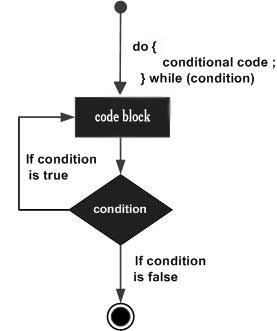
\includegraphics[width=0.4\linewidth]{P2/img/dowhileloop.png}
	\caption{Pernyataan do-while}
	\label{fig:dowhileloop}
\end{figure}
Syntaxnya pada bahasa C adalah sebagai berikut:
% Its syntax in C is as follows:
\begin{verbatim}
    do{
        // the block of code that will be repeated
    }while(Condition)
\end{verbatim}
Sebagai contoh, perhatikan kode berikut
% Look at the following example.
\begin{lstlisting}[language=c,caption = Contoh Penggunaan do-while,label=lst:dowhileexample01]
int main()
{
	int uangSaya,hargaRoti;
	uangSaya = 10000;
	hargaRoti = 12000;
	do{
	    printf("Beli roti 1, uang saya sisa %d", uangSaya - hargaRoti);
	    uangSaya -= hargaRoti;
	}while(uangSaya >= hargaRoti)
	printf("Uang saya tidak cukup lagi");
	return 0;
}
\end{lstlisting}
Output dari program pada Listing \ref{lst:dowhileexample01} adalah
% The output of the code above are
\begin{verbatim}
    Beli roti 1, uang saya sisa -2000
    Uang saya tidak cukup lagi
\end{verbatim}
% The variable \verb|uangSaya| is substracted by \verb|hargaRoti| before checking the \verb|uangSaya>=hargaRoti| condition.
% Had the code above uses while loop, the repeating block of code wouldn't have executed even once.
Variabel \verb|uangSaya| dikurangi dengan \verb|hargaRoti| sebelum memeriksa \verb|uangSaya>=hargaRoti| kondisi.
Seandainya kode di atas menggunakan perulangan while, blok kode yang berulang tidak akan dieksekusi sekali pun.
\subsection{Perulangan for}
Misalkan terdapat blok kode while dengan bentuk seperti ini:
% If you have a block of code like this:
\begin{verbatim}
    InitializationStatement; // e.g.: int i = 0;
    while(Condition){
        // do something
        updateStatement; // e.g.: i++ 
    }
\end{verbatim}
Hal ini setara dengan
\begin{verbatim}
    for(InitializationStatement;Condition;updateStatement){
        // do something
    }
\end{verbatim}

Sebagai contoh, perhatikan program berikut:
% As example, look at the following code:
\begin{lstlisting}[language=c,caption = Contoh Penggunaan for,label=lst:forexample01]
int main()
{
    int i=0;
    for(i=1;i<10;i++){
        printf("%d ",i);
    }
	return 0;
}
\end{lstlisting}
Output dari program ini adalah
% The output of this program are
\begin{verbatim}
    1 2 3 4 5 6 7 8 9 
\end{verbatim}
Berikut kode pada Listing \ref{lst:forexample01} jika diubah menjadi bentuk while-loop
% The following is the code if code in Listing \ref{lst:forexample01} converted to its while-loop form
\begin{lstlisting}[language=c,caption = For dalam bentuk while,label=lst:forwhileform01]
int main()
{
    int i=0;
    i=1;
    while(i<10){
        printf("%d ",i);
        i++;
    }
	return 0;
}
\end{lstlisting}
\begin{center}
	\colorbox{pink}{\parbox{0.8\linewidth}{\textbf{Catatan:} Terdapat keyword break dan continue digunakan untuk mengendalikan (kontrol) alur pada perulangan. Pelajari secara mandiri!}}
\end{center}

\subsection{Tugas Pendahuluan}
\begin{enumerate}
	\item Implementasikan program dalam bahasa C yang menghitung faktorial dari sebuah bilangan bulat non-negatif yang dimasukkan oleh pengguna menggunakan loop do-while. Tampilkan hasilnya.
	\item Implementasikan program dalam bahasa C untuk mencari bilangan prima antara 1 dan 100. Gunakan loop for untuk mengiterasi melalui semua angka dan pernyataan continue untuk mengabaikan angka yang bukan prima. Tampilkan semua bilangan prima yang ditemukan.
\end{enumerate}

\section{Array}
Array atau biasa disebut larik adalah koleksi data dimana setiap elemen mempunyai nama yang sama dan bertipe sama. Setiap elemen diakses berdasarkan  indeks elemennya.
% Array is a collection of data where each element of it has the same name(indexed) and data type. Every element in an array can be accessed using its element index.
\subsection{Array 1D}
Variabel array dimensi satu dideklarasikan dengan menentukan jenis elemen dan jumlah elemen yang di perlukan oleh array.
% One dimensional array variable can be declared by deciding the data type of the element and the number of element that is needed.

Syntax:
\begin{verbatim}
    DataType variableName [arraySize];
\end{verbatim}
\begin{enumerate}
	\item \verb*|DataType|.\\
	      % The data type of the elements in the array, e.g. \verb|float|, \verb|int|, etc.
	      Jenis elemen data elemen array :\verb*|float|,\verb*|int|,\verb*|char| dsb
	\item \verb*|variableName|\\
	      Namariabel mengikuti aturan pemberian nama variabel,
	      % variableName follows the variable naming convention

	\item \verb*|arraySize| \\
	      % Integer more than 0. Defining the number of element an array has.
	      konstanta integer lebih besar dari 0. \\
\end{enumerate}

Untuk menginisialisasi array dimensi satu, dapat dilakukan dengan cara seperti berikut:
% Initializing one dimensional array can be done like shown below:
\begin{verbatim}
    int contoh_array[5] = {4,2,0,6,9};
\end{verbatim}

Data di dalam array dapat akses dengan menggunakan suatu bilangan yang merupakan index dari array tersebut. Perhatikan potongan kode berikut.
% Data in an array can be accessed by using an integer that is the index of the array. Look at the code below

\begin{lstlisting}[language=c,caption = Contoh Mengakses Array 1D,label=lst:array1d01]
int main()
{
    int arr[5] = {4,2,0,6,9};
    printf("%d\n",arr[0]);
    printf("%d\n",arr[4]);
    int i = 0;
    printf("%d\n",arr[i]);
    for(i=0;i<5;i++)
        printf("%d",arr[i]);
}
\end{lstlisting}

Potongan kode pada Listing \ref{lst:array1d01} akan memberikan output
% The code in Listing \ref{lst:array1d01} will give output
\begin{verbatim}
    4
    9
    4
    42069
\end{verbatim}

\subsection{Array 2D dan Array Multidimensi lainnya}%Array 2D dan Array Multidimensi lainnya}
Array dimensi dua pada dasarnya hanya merupakan array dimensi satu dari array dimensi satu. Oleh karena itu, untuk mendeklarasikan array dimensi dua kita dapat menggunakan syntax seperti berikut.
% 2D array is basically a 1D array of 1D array. Intuitively, you can define a 2D array like as seen below:
\begin{verbatim}
	DataType variableName[arraySize1][arraySize2];
\end{verbatim}
Hal ini berlaku juga untuk array dengan dimensi lebih dari dua.
% This also applies to multidimensional array.
\begin{verbatim}
    DataType variableName[arraySize1]...[arraySizeN];
\end{verbatim}
Akan ada $arraySize_1\times arraySize_2 \times \cdots \times arraySize_n$ elemen yang akan dialokasikan ke memori setelah melakukan array multidimensi seperti itu
% There will be $arraySize_1\times arraySize_2 \times \cdots \times arraySize_n$ of elements that would be allocated to the memory after doing multidimensional array like that.

Untuk menginisialisasi suatu array multidimensi dapat dilakukan sama seperti array biasa:
% To initialize multidimensional array, you can do the following:
\begin{verbatim}
    int arr[2][2] = {{1,2},{3,4}};
\end{verbatim}

\subsection{Tugas Pendahuluan}
\begin{enumerate}
	\item Cobalah inisialisasi suatu array multidimensi dengan menggunakan perulangan for.
	      % \item Try to initialize a multidimensional array with for loop
	\item Buatlah suatu program untuk mengisi data pada suatu array perdasarkan input dari keyboard.
	      % \item create a program to fill the data of an array by keyboard input.
	\item Apakah yang akan terjadi jika suatu array \verb|arr| diakses dengan \verb|arr[-1]|?
	      % \item What would happen if an array \verb|arr| is accessed with \verb|arr[-1]|?
	\item Apakah yang akan terjadi jika suatu array \verb|arr| dengan ukuran 5 diakses dengan \verb|arr[5]|?
	      % \item What would happen if an array \verb|arr| with size 5 is accessed with \verb|arr[5]|?
	\item Lihatlah kode berikut
	      % \item Look at the following code
	      \begin{verbatim}
        for(i=0;i<10;i++){
            for(j=i;j<10;j++){
                printf("A");
            }
        }
    \end{verbatim}
	      % How many "A" will be printed on the screen if that block of code is executed?
	      Ada berapa banyakah huruf A yang akan muncul pada layar jika program tersebut dijalankan?
\end{enumerate}

\section{String}
Secara umum, string merupakan kumpulan dari satu atau lebih karakter. Spesifik pada bahasa C, string didefinisikan sebagai kumpulan karakter yang diakhiri oleh karakter null \verb|'\0'|.
\\
Misalkan string  \verb|"Dasar"|, pada bahasa C direpresentasikan sebagai kumpulan karakter \verb|'D'|, \verb|'a'|, \verb|'s'|, \verb|'a'|, \verb|'r'|, dan \verb|'\0'|.

\subsection{Penggunaan String}
Karena string tidak lain adalah array dari char, maka cara pembuatan tipe data string dalam bahasa C juga sama seperti cara pembuatan array. Berikut contohnya:
\begin{lstlisting}[language=c,caption = Contoh String dari Char,label=lst:array1d01]
	#include <stdio.h>
 
	int main(void)
	{
	char foo[8] = {'b','e','l','a','j','a','r','\0'};
	printf("Isi variabel foo adalah %s \n", foo);
	
	return 0;
	}
\end{lstlisting}

\verb|‘\0’| adalah salah satu syarat pembuatan string di dalam bahasa C.
Semua string harus memiliki karakter “khusus” untuk menandakan akhir dari string.
Tanda \verb|‘\0’| mewakili karakter null yang dipakai oleh compiler bahasa C sebagai tanda akhir sebuah string.

Contoh source code penggunaan \verb|scanf| untuk membaca string:
\begin{lstlisting}[language=c,caption = Contoh String dengan scanf,label=lst:scanf]
	#include <stdio.h>

	int main() {
		// Mendeklarasikan variabel untuk menyimpan input dari pengguna
		int age;
		float height;
		char name[50];

		// Meminta pengguna untuk memasukkan usia mereka
		printf("Masukkan usia Anda: ");
		scanf("%d", &age);
		
		// Meminta pengguna untuk memasukkan tinggi mereka
		printf("Masukkan tinggi Anda (dalam meter): ");
		scanf("%f", &height);
		
		// Meminta pengguna untuk memasukkan nama mereka
		printf("Masukkan nama Anda: ");
		scanf("%s", name);

		// Menampilkan informasi yang dimasukkan pengguna
		printf("Nama: %s\n", name);
		printf("Usia: %d tahun\n", age);
		printf("Tinggi: %.2f meter\n", height);

		return 0;
	}
\end{lstlisting}


Contoh source code penggunaan \verb|gets| untuk membaca string:
\begin{lstlisting}[language=c,caption = Contoh String dengan gets,label=lst:gets]
#include <stdio.h>

int main () {
  
	char arr[100];
	while(true)
	{
		gets(arr);
		
		printf("-- %s\n", arr);
	}
  return 0;

}
\end{lstlisting}

String yang dibaca dengan mengunakan scanf atau gets akan secara otomatis memiliki \verb|null| character di akhir.

\subsection{Fungsi-Fungsi String}
Dalam bahasa pemrograman C, terdapat library yang dibuat dengan tujuan memudahkan pengguna dalam mengolah string.
Library tersebut tersimpan dalam \verb|<string.h>|,
oleh karena itu, untuk mengakses library ini, diperlukan tambahan preprocessor, yaitu:
\begin{lstlisting}[language=c]
	#include <string.h>
\end{lstlisting}

Pelajari berbagai fungsinya di \href{http://www.cplusplus.com/}{www.cplusplus.com}.

\subsection{Tugas Pendahuluan}
\begin{enumerate}
	\item Buatlah program dalam bahasa C yang mengambil dua string dari pengguna dan menentukan apakah kedua string tersebut anagram (mengandung karakter yang sama dalam urutan yang berbeda).
	      Tampilkan pesan yang sesuai.
	\item Jelaskan perbedaan antara string yang dideklarasikan sebagai array karakter (char array) dan string yang dideklarasikan sebagai tipe data string (string literal) dalam bahasa C. Berikan contoh penggunaan keduanya.
\end{enumerate}
 % \chapter{Fungsi (Subprogram)}
\section*{Tujuan}
\begin{itemize}[label=$\bullet$, itemsep=-1pt, leftmargin=*]
    % \item Students understand how to create and call functions in C .
    \item Mahasiswa mengerti cara membuat dan memanggil fungsi pada bahasa pemrograman C.
          % \item Students able to pass parameter by value and by reference in C.
    \item Mahasiswa mampu menggunakan passing parameter by value dan by reference pada bahasa pemrograman C.
          % \item Students understand and able to apply recursion in C. 
    \item Mahasiswa mampu mengerti dan mengaplikasikan konsep rekursi pada bahasa pemrograman C.
\end{itemize}

\section{Fungsi}

Fungsi adalah blok kode bernama yang dibuat untuk melakukan tugas tertentu.
Fungsi membantu membuat program lebih modular, rapi, dan mudah dipelihara.
Setiap fungsi dapat dipanggil berulang kali dari bagian program manapun tanpa menulis ulang kode.
\\\\Manfaat fungsi
\begin{enumerate}
    \item \textbf{Mengurangi Duplikasi Kode} \\
    Jika ada perintah yang sama dipakai berulang, cukup ditulis satu kali di dalam fungsi.
    Tinggal dipanggil kapanpun dibutuhkan.
    \item \textbf{Meningkatkan Keterbacaan dan Struktur Program} \\
    Program dengan fungsi lebih mudah dibaca dan dipahami karena tersusun rapi.
    Nama fungsi juga bisa mendeskripsikan tugasnya.
    \item \textbf{Memudahkan Pemeliharaan (Maintenance)} \\
    Jika ada perubahan, cukup memperbarui fungsi terkait tanpa harus mengubah seluruh kode program.
    \item \textbf{Dapat Digunakan Kembali (Reusability)} \\
    Fungsi bisa dipakai kembali di program lain dengan sedikit atau tanpa modifikasi.
    \item \textbf{Memudahkan Debugging dan Testing} \\
    Kesalahan lebih mudah dilacak karena fungsi bisa diuji satu per satu.
\end{enumerate}
Berdasarkan sumbernya, fungsi dibedakan menjadi dua, yaitu:
\begin{enumerate}
    \item \textbf{Fungsi library (Predefined function)} \\
    Fungsi yang sudah tersedia dalam bahasa C, seperti main(), printf() dan scanf().
    Fungsi ini berasal dari sebuah library yang dimasukkan dengan header file seperti \verb|#include <stdio.h>|.
    \item \textbf{Fungsi buatan sendiri (User-defined function)} \\
    Fungsi ini dibuat oleh programmer sendiri sesuai kebutuhan.
\end{enumerate}

\subsection{Membuat fungsi}

Untuk membuat fungsi kita bisa menuliskan:
{
\captionsetup[lstlisting]{labelformat=empty, justification=raggedright, singlelinecheck=false} %agar caption tanpa label dan di kiri
\begin{lstlisting}[language=c, caption={syntax}]
    tipe_data nama_fungsi(parameter){
    // kode yang akan dijalankan ketika fungsi dipanggil
    }
\end{lstlisting}
}
\begin{enumerate}[label={}, leftmargin=*]
    \item \verb|tipe_data|: tipe data untuk nilai kembalian fungsi (jika tidak ada nilai kembali bisa menggunakan tipe data void).
    \item \verb|nama_fungsi|: nama dari fungsi.
    \item \verb|parameter|: nilai atau variabel yang dimasukkan ke dalam fungsi.
\end{enumerate}

\subsubsection{Deklarasi dan definisi fungsi}

Sebuah fungsi terdiri dari dua bagian, yaitu:
Deklarasi: berisi tipe data nilai kembalian, nama fungsi, dan parameter.
Definisi: berisi kode yang akan dijalankan ketika fungsi dipanggil.
Contoh:
\begin{lstlisting}[language=c]
	void fungsi(int angka){ // Deklarasi
	// kode (Definisi)
	}
\end{lstlisting}
Pada contoh di atas, deklarasi dan definisi ditulis bersamaan.
Kita juga bisa menulis deklarasi dan definisi secara terpisah agar kode lebih mudah terbaca.
Untuk melakukannya kita tulis deklarasi di atas fungsi main(), dan definisi di bawah fungsi main().
Contoh:
\begin{lstlisting}[language=c]
	// Deklarasi
	void fungsi(int angka);

	//fungsi main
	int main(){

	}

	// Definisi
	void fungsi(int angka){

	}
\end{lstlisting}

\subsection{Memanggil fungsi}

Untuk menggunakan fungsi yang sudah dibuat, kita perlu memanggil fungsi tersebut.
Untuk memanggil sebuah fungsi, tulis nama fungsinya dan tanda kurung "()".
Contoh:
\begin{lstlisting}[language=c]
	void halo(){
		printf("Halo dunia!");
	}

	int main(){
		halo();
		return 0;
	}
\end{lstlisting}
\begin{verbatim}
	Output:
	Halo dunia!
\end{verbatim}
Sebuah fungsi bisa dipanggil berkali-kali. Contoh:
\begin{lstlisting}[language=c]
	void halo(){
		printf("Halo dunia!\n");
	}

	int main(){
		halo();
		halo();
		halo();
		return 0;
	}
\end{lstlisting}
\begin{verbatim}
	Output:
	Halo dunia!
	Halo dunia!
	Halo dunia!
\end{verbatim}

\subsection{Parameter dan Argumen}

Parameter adalah variabel yang didefinisikan ketika deklarasi atau definisi.
Parameter digunakan agar fungsi bisa menerima data dari luar fungsi.
Contoh:
\begin{lstlisting}[language=c]
	void jumlah(int a, int b){
		printf("%d", a+b);
	}
\end{lstlisting}
Fungsi di atas memiliki parameter dua angka integer a dan b.
Kedua parameter ini bisa digunakan di dalam fungsi, dalam contoh di atas dilakukan operasi penjumlahan dan menampilkan hasilnya.
\\ Nilai yang dikirimkan ke parameter adalah sebuah argumen.
Contoh:
\begin{lstlisting}[language=c]
	void jumlah(int a, int b){
		printf("%d", a+b);
	}

	int main(){
		jumlah(10, 5);

		return 0;
	}
\end{lstlisting}
\begin{verbatim}
	Output:
	15
\end{verbatim}
Dari contoh di atas, int a dan int b merupakan parameter, 10 dan 5 adalah argumen.
Ketika fungsi di atas dipanggil, nilai dari parameter a adalah 10, dan b adalah 5, sehingga menghasilkan output 15.

\subsection{Nilai kembalian}

Nilai kembalian adalah hasil yang dikirimkan oleh sebuah fungsi kepada bagian program yang memanggil fungsi tersebut.
Nilai kembalian harus sesuai dengan tipe data dari fungsi itu sendiri.
Fungsi dengan tipe void tidak memiliki kembalian.
Nilai kembalian ditentukan dengan keyword return.
contoh:
\begin{lstlisting}[language=c]
#include <stdio.h>

int tambah(int a, int b) {
	return a + b;  // mengembalikan hasil penjumlahan
}

int main(){
	int a = 5, b = 10;
	int jumlah = tambah(a, b); // nilai kembalian disimpan ke variabel
	printf("%d", jumlah);
}
\end{lstlisting}
Dari contoh diatas, nilai kembalian dari fungsi tambah() adalah penjumlahan kedua parameternya.
Nilai kembalian tersebut bisa didapatkan ketika fungsi dipanggil seperti pada baris 8.

\subsection{Scope variabel}

Dalam pemrograman, variabel memiliki scope atau jangkauan dimana variabel bisa diakses.
Contoh:
\begin{lstlisting}[language=c]
	void nilai(){
		int x = 1;
	}

	int main(){
		nilai();
		printf("%d", x);

		return 0;
	}
\end{lstlisting}
Dari contoh di atas, meskipun variable x sudah dideklarasi di dalam fungsi nilai().
Ketika variabel tersebut diakses di luar fungsi, akan terjadi error karena variabel x hanya bisa diakses di dalam fungsi.

\subsubsection{Variabel lokal}

Variabel lokal adalah variabel yang dideklarasikan di dalam fungsi atau sebuah blok kode (di dalam tanda kurung kurawal '{}').
Variabel ini hanya bisa diakses blok kode tempat variabel tersebut dideklarasikan.
Contoh:
\begin{lstlisting}[language=c]
#include <stdio.h>

int main(){
	int x = 10; //deklarasi variabel x

	if(x>9){
		int y = 10; //deklarasi variabel y`
		x = 0; // akses variabel x
	}
	printf("%d\n", x); // akses variabel x
	printf("%d\n", y); // akses variabel y.

	return 0;
}
\end{lstlisting}
Dari contoh di atas, variabel x dideklarasikan di dalam fungsi main, sehingga di dalam fungsi main().
Jadi variabel x bisa kita akses seperti pada baris 8 dan 10, karena masih di dalam fungsi main().
Sedangkan variabel y dideklarasikan di dalam fungsi if().
Jadi jika kita akses seperti pada baris 11 akan terjadi error, karena baris 11 berada di luar fungsi if().

\subsubsection{Variabel Global}

Variabel global adalah variabel yang dideklarasikan di luar semua fungsi.
Variabel ini bisa diakses dari semua tempat di dalam program.
Contoh:
\begin{lstlisting}[language=c]
#include <stdio.h>

int x = 1; // deklarasi global

void ubah(){
	x = 5; // akses di dalam fungsi, akan dieksekusi ketika fungsi dipanggil
}

int main(){
	printf("%d\n", x); // akses di main()
	x = 2;
	printf("%d\n", x);

	ubah(); // akses variabel x dari dalam fungsi.

	printf("%d\n", x);
	return 0;
}
\end{lstlisting}
\begin{verbatim}
	Output:
	1
	2
	5
\end{verbatim}
Dari contoh di atas, variabel x adalah variabel global yang mana bisa diakses dari fungsi main() maupun fungsi ubah().

\subsubsection{Penamaan variabel}

Jika variabel global dan variabel lokal memiliki nama yang sama, 
bahasa C akan menganggap kedua variabel tersebut sebagai dua variabel yang berbeda.
Contoh:
\begin{lstlisting}[language=c]
#include <stdio.h>

int x = 1; deklarasi global

void angka(){
	int x = 5; // deklarasi lokal
	printf("%d\n", x); // akses variabel lokal
}

int main(){
	angka();

	printf("%d\n", x); // akses variabel global

	return 0;
}
\end{lstlisting}
\begin{verbatim}
    Output:
    5
    1
\end{verbatim}
Variabel x dideklarasikan secara global dan secara lokal di dalam fungsi angka().
Sehingga ketika mengakses variabel x di dalam fungsi angka(), yang diakses adalah variabel lokal, bukan global.

\subsection*{Tugas Pendahuluan 1}
\begin{enumerate}
    \item Fungsi dapat membuat program lebih efisien dan mudah dibaca, jelaskan alasannya!
    \item Apa itu variabel statis? Jelaskan apa saja kegunaannya!
    \item Berikan contoh masalah yang akan lebih mudah diselesaikan dengan menggunakan fungsi!
    \item Buatlah sebuah fungsi yang mengembalikan nilai akar sebuah angka! (jangan gunakan fungsi library).
\end{enumerate}

\section{Rekursi}

Rekursi adalah teknik dimana sebuah fungsi memanggil dirinya sendiri.

\subsection{Struktur Rekursi}

Rekursi terbagi menjadi dua bagian
\begin{enumerate}
    \item \textbf{Kasus dasar (base case)} \\
    Sebuah kondisi yang membuat rekursi berhenti.
    Digunakan agar tidak terjadi rekursi terus-menerus.
    \item \textbf{Kasus rekursi (recursive case)} \\
    Bagian dimana fungsi memanggil dirinya sendiri.
\end{enumerate}

\subsection{Contoh penggunaan rekursi}

\begin{lstlisting}[language=c]
#include <stdio.h>

int faktorial(int n) {
	if (n == 0 || n == 1)  // base case
	return 1;
	else                   // recursive case
	return n * faktorial(n - 1);
}

int main() {
	printf("5! = %d\n", faktorial(5));
	return 0;
}
\end{lstlisting}
Contoh di atas adalah penggunaan rekursi untuk menghitung nilai faktorial.
Fungsi faktorial(n) akan mengembalikan nilai n x faktorial(n-1), lalu faktorial(n-1) akan mengembalikan nilai n-1 x faktorial(n-2), dan seterusnya.
Hal ini akan berulang terus menerus hingga kondisi base case terpenuhi yaitu ketika nilai n adalah 0 atau 1.
\begin{verbatim}
    faktorial(n) = n x faktorial(n-1)
                 = n x n-1 x faktorial(n-2)
                 = n x n-1 x n-2 x faktorial(n-3)
                 = n x n-1 x n-2 x ... x 2 x faktorial(1)
                 = n x n-1 x n-2 x ... x 2 x 1
\end{verbatim}

\subsection*{Tugas Pendahuluan 2}
\begin{enumerate}
    \item Berikan contoh masalah apa yang lebih mudah diselesaikan menggunakan rekursi!
    \item Apa saja kelebihan dan kekurangan dari rekursi? jelaskan!
    \item Perhatikan kode berikut:
    \begin{lstlisting}[language=c]
	int faktorial(int n) {
		if (n == 0 || n == 1)  // base case
		return 1;
		else                   // recursive case
		return n * faktorial(n - 1);
	}
\end{lstlisting}
   Jika ketika fungsi dipanggil kita masukkan argumen berupa angka negatif, apa yang terjadi?
   Apa solusi yang bisa kamu berikan?
    \item Pelajarilah algoritma searching! Tuliskan apa saja yang kamu pelajari!
    \item Algoritma searching apa yang paling efisien? kenapa?
\end{enumerate}
% \section{Tujuan}
\begin{itemize}[label=$\bullet$, itemsep=-1pt, leftmargin=*]   
    \item Mahasiswa mengerti tentang konsep pointer pada bahasa pemrograman C.
    \item Mahasiswa mengerti cara membuat dan memanggil struct pada bahasa pemrograman C.
    \item Mahasiswa mengerti tentang algoritma sorting pada bahasa pemrograman C.
    \item Mahasiswa mengerti tentang algoritma searching pada bahasa pemrograman C.
    \item Mahasiswa mampu mengaplikasikan konsep algoritma searching dan sorting pada bahasa pemrograman C.
\end{itemize}

\section{Pointer}
\subsection{Alamat Memori}
Setiap variabel, fungsi, struct, ataupun objek lain yang dibuat dalam program mempunyai lokasi masing-masing pada memori. Alokasi setiap variabel disimpan dalam alamat memori tertentu.

Jika  terdapat variabel \verb|var| di program Anda, \verb|&var| akan memberi alamatnya di memori.
\begin{lstlisting}[language=c]
    int var = 5;
    printf("%d\n", var);
    printf("%p\n", &var);
\end{lstlisting}
\begin{center}
	\colorbox{pink}{\parbox{0.8\linewidth}{\textbf{Catatan:} Output bisa berbeda-beda di tiap eksekusi.}}
\end{center}

\subsection{Pengenalan Pointer} 

Pointer (variabel penunjuk) adalah variabel khusus yang digunakan untuk menyimpan alamat, bukan nilai.

Deklarasi variabel pointer menggunakan operator \verb|*| di antara tipe data dan nama variabelnya.
\begin{lstlisting}[language=c]
	#include <stdio.h>
int main()
{
	int* p; // atau
    int * p2;
	return 0;
}
\end{lstlisting}


\subsection{Cara Kerja Pointer}
Berikut adalah cara kerja dari pointer.
\begin{lstlisting}[language=c, caption={Contoh Program Pointer}]
    #include <stdio.h>
    int main()
    {
       int* pc, c;
       
       c = 22;
       printf("Address of c: %p\n", &c);
       printf("Value of c: %d\n\n", c);  // 22
       
       pc = &c;
       printf("Address of pointer pc: %p\n", pc);
       printf("Content of pointer pc: %d\n\n", *pc); // 22
       
       c = 11;
       printf("Address of pointer pc: %p\n", pc);
       printf("Content of pointer pc: %d\n\n", *pc); // 11
       
       *pc = 2;
       printf("Address of c: %p\n", &c);
       printf("Value of c: %d\n\n", c); // 2
       return 0;
    }
\end{lstlisting}

Penjelasan Program:\\
\begin{enumerate}
    \item \verb|int* pc, c;|
    \begin{figure}[H]
        \centering
        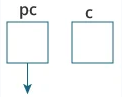
\includegraphics[width=0.2\linewidth]{../P4/img/screenshot001.png}
        \caption{}
        \label{fig:satu}
    \end{figure}
    \item \verb|c = 22;|
    \begin{figure}[H]
        \centering
        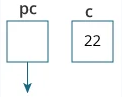
\includegraphics[width=0.2\linewidth]{../P4/img/screenshot002.png}
        \caption{}
        \label{fig:dua}
    \end{figure}
    \item \verb|pc = &c;|
    \begin{figure}[H]
        \centering
        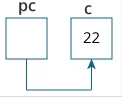
\includegraphics[width=0.2\linewidth]{../P4/img/screenshot003.png}
        \caption{}
        \label{fig:tiga}
    \end{figure}
    \item \verb|c = 11;|
    \begin{figure}[H]
        \centering
        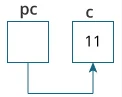
\includegraphics[width=0.2\linewidth]{../P4/img/screenshot004.png}
        \caption{}
        \label{fig:empat}
    \end{figure}
    \item \verb|*pc = 2;|
    \begin{figure}[H]
        \centering
        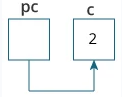
\includegraphics[width=0.2\linewidth]{../P4/img/screenshot005.png}
        \caption{}
        \label{fig:lima}
    \end{figure}
\end{enumerate}

\subsection{Double Pointer}
Variabel pointer juga dapat menunjuk variabel pointer lainnya. 
Hal ini disebut dengan double pointer (pointer to pointer). 
Untuk mendeklarasikan variabel double pointer, digunakan dua simbol *. 
Kegunaan paling umum dari variabel double pointer adalah untuk membuat array dua dimensi secara dinamis.
\begin{lstlisting}[language=c]
    int **dbPtr;
\end{lstlisting}
Variabel dbPtr di atas menyimpan alamat memori dari variabel pointer lainnya. \\
Berikut contohnya
\begin{lstlisting}[language=c,  caption={Contoh Double Pointer}]
#include <stdio.h>

int main(void)
{
    int var = 23;
    int *ptr = &var;
    int **dbPtr = &ptr;

    printf("%d\n", **dbPtr);
        
    return 0;
}
\end{lstlisting}

\subsection{Tugas Pendahuluan}
\begin{enumerate}
   \item Bagaimana cara mendeklarasikan pointer ke array multidimensi?
   \item Buatlah program dalam bahasa C atau C++ yang mengimplementasikan 
   fungsi void printMatrix(int **matrix, int rows, int cols) untuk mencetak matriks 2D menggunakan pointer ke pointer. Lalu, dalam fungsi main, 
   buatlah matriks 2D dan panggil fungsi printMatrix untuk mencetak matriks tersebut.
\end{enumerate}

\section{Struct}
Dalam pemrograman C, struct (atau struktur) adalah kumpulan variabel (bisa dari tipe berbeda) di bawah satu nama. 
Tidak seperti array yang hanya dapat menyimpan elemen dengan tipe data sama, 
struct dapat mengelompokkan elemen dengan tipe data yang berbeda-beda.


\subsection{Deklarasi Struct}
Seperti variabel, struct harus dideklarasikan terlebih dahulu sebelum bisa digunakan. Pendeklarasian struct menggunakan sintaks sebagai berikut.

\begin{lstlisting}[language=c]
struct <nama_struct> {
    <tipe_data_member> <nama_member>;
    <tipe_data_member> <nama_member>;
    <tipe_data_member> <nama_member>;
    .
    .
    .
};
\end{lstlisting}

Berikut adalah contoh deklarasi struct berdasarkan kasus Mahasiswa.
\begin{lstlisting}[language=c]
struct Mahasiswa
{
    char *name;
    char *address;
    int age;
};
\end{lstlisting}
\begin{center}
	\colorbox{pink}{\parbox{0.8\linewidth}{\textbf{Catatan:}  Menggunakan pointer * untuk data string}}
\end{center}

Setelah dideklarasikan, sebuah struct akan menjadi tipe data baru. 
Maka dalam kasus ini, struct Mahasiswa di sini menjadi tipe data baru dengan member-member berupa \verb|nama|, \verb|address|, dan \verb|age|. 
Untuk membuat variabel dengan tipe data struct, dilakukan dengan sintaks berikut.

\begin{lstlisting}[language=c]
    struct <nama_struct> <nama_variabel>;
\end{lstlisting}

Contoh:
\begin{lstlisting}[language=c]
    struct Mahasiswa mhs1;
    struct Mahasiswa mhs2;
\end{lstlisting}
Contoh di atas menunjukkan terdapat dua variabel \verb|mhs1| dan \verb|mhs2 |bertipe struct \verb|Mahasiswa|.

\subsection{Akses Member Struct}
Bagaimana cara untuk mengakses member dari variabel struct yang telah dibuat? \\
Untuk mengakses member-member dari struct, digunakan operator dot (.) setelah nama variabelnya.
\begin{lstlisting}[language=c]
    <nama_variabel>.<member_struct>
\end{lstlisting}

Contoh:
\begin{lstlisting}[language=c]
    mhs1.age = 20;
    mhs1.nama = iqbal;
    
    mhs2.nama = fatur;
    mhs2.age = 21;
\end{lstlisting}

\subsection{Tugas Pendahuluan}
\begin{enumerate}
    \item Buatlah sebuah struct yang merepresentasikan informasi tentang seorang mahasiswa, yang memiliki nama, nim, dan nilai IPK. Kemudian, buatlah program untuk menginput data mahasiswa, menampilkan data mahasiswa, dan menghitung rata-rata IPK dari sejumlah mahasiswa.
    \item Anda diberikan struct yang merepresentasikan titik dalam sistem koordinat dua dimensi (x, y). Buatlah sebuah program C untuk menghitung jarak antara dua titik yang diinputkan oleh pengguna menggunakan rumus jarak Euclidean.
\end{enumerate}

\section{Algoritma Sorting}
Sorting merupakan suatu proses penyortiran atau pengurutan sebuah data.\\
Terdapat 2 macam pengurutan data pada sorting yaitu :
\begin{enumerate}
    \item Berdasarkan ascending (kecil ke besar).
    \item Berdasarkan Descending (besar ke kecil).
\end{enumerate}

\subsection{Bubble Sort}
Bubble sort merupakan algoritma pengurutan yang membandingkan dua data yang berdekatan dan menukarnya sampai tidak dalam urutan yang diinginkan.
Bubble sort menggunakan teknik iterasi. Iterasi merupakan proses melakukan perulangan sebanyak data yang diketahui.
Intinya pada iterasi melakukan perbandingan antara dua data.

\begin{figure}[H]
    \centering
    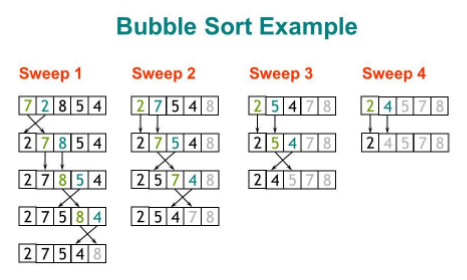
\includegraphics[width=0.7\linewidth]{../P4/img/screenshot006.png}
    \caption{}
    \label{fig:enam}
\end{figure}

\begin{lstlisting}[language=c,caption=Implementasi Bubble Sort]
void swap ( int * xp , int * yp ) {
   int temp = *xp;
   *xp = *yp;
   *yp = temp;
}

void bubbleSort(int arr[], int n) {
   int i, j, swapped;        // dioptimasi dengan bool `swapped`:
   for (i = 0; i < n-1; i++) {
      swapped = 0;
      for (j = 0; j < n-i-1; j++) {
         if (arr[j] > arr[j+1]) {
            swap(&arr[j], &arr[j+1]);
            swapped = 1;
         }
      }
      if (swapped == 0)
         break;
   }
}
\end{lstlisting}

\subsection{Insertion Sort}
Insertion sort merupakan teknik sorting dengan cara menyisipkan atau memasukan setiap elemen secara berulang berulang.
Konsep insertion sort bisa diibaratkan sebuah kartu. 

\begin{figure}[H]
    \centering
    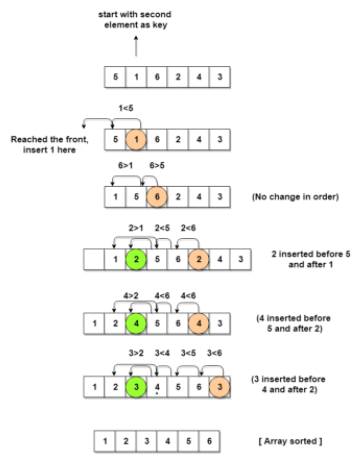
\includegraphics[width=0.5\linewidth]{../P4/img/screenshot007.png}
    \caption{}
    \label{fig:tujuh}
\end{figure}
\begin{lstlisting}[language=c,caption=Implementasi Insertion Sort], 
void insertionSort(int arr[]. int n) {
   int i, key, j;
   for (i = 1; i < n; i++) {
      key = arr[i];
      j = i-1;
    
      while (j >= 0 && arr[j] > key) {
         arr[j+1] = arr[j];
         j = j-1;
      }
      arr[j+1] = key;
   }
}
\end{lstlisting}

\begin{center}
	\colorbox{pink}{\parbox{0.8\linewidth}{\textbf{Catatan:} Terdapat berbagai algoritma sorting lain. Pelajari secara mandiri}}
\end{center}

\subsection{Tugas Pendahuluan}
\begin{enumerate}
    \item Urutkan array berikut menggunakan algoritma Bubble Sort:

    Array: [5, 2, 9, 1, 5, 6]
    \item Hitung kompleksitas waktu (Big O) dari algoritma Insertion Sort saat mengurutkan sebuah array dengan panjang n, dan jelaskan bagaimana kompleksitas ini dihitung.
\end{enumerate}

\section{Algoritma Searching}
Searching merupakan proses pencarian sebuah data yang diinginkan.

\subsection{Linear Search}
Linear Search bekerja dengan melakukan pengecekan kepada semua elemen yang ada.\\
Secara garis besar, cara kerja Linear Search adalah:

\begin{enumerate}
    \item Memeriksa item satu per satu.
    \item Apabila ditemukan, maka “ketemu”.
    \item Jika sampai akhir belum ditemukan, maka item yang dicari tidak ada.
\end{enumerate}

\begin{lstlisting}[language=c,caption=Implementasi Linear Search], 
int linearSearch(int arr[], int n, int item) {
    int i;
    for(i = 0; i < n; ++i) {
        if(item == arr[i])
          return 1;
    }
    return -1;
}
\end{lstlisting}   

\subsection{Binary Search}
Binary Search adalah teknik pencarian di mana untuk setiap iterasinya kita membagi space pencarian menjadi hanya setengah 
dari space pencarian awal hingga kita menemukan yang kita cari.    

\begin{lstlisting}[language=c,caption=Implementasi Binary Search],   
bool f(int k, int a, int b, int n) {
   return ((k/a) * (b/a) >= n);
}

int binser(int a, int b, int n) {
   int l = 1;
   int r = 100000;
   while (r - l > 1) {
      int mid = (l + r) >> 1;
      bool can = f(mid);
      if(can)
         r = mid;
      else
         l = mid + 1;
   }
   if (can(l))
      return l;
   else
      return r;
}
\end{lstlisting}

\begin{center}
	\colorbox{pink}{\parbox{0.8\linewidth}{\textbf{Catatan:} Terdapat berbagai algoritma searching lain. Pelajari secara mandiri}}
\end{center}

\subsection{Tugas Pendahuluan}
\begin{enumerate}
    \item Anda memiliki daftar nama berikut: ["Alice", "Bob", "Charlie", "David", "Eve", "Frank"]. 
    Gunakan algoritma binary search untuk mencari apakah nama "Eve" ada dalam daftar ini. 
    Jika ya, berapa langkah yang dibutuhkan?
    \item Jelaskan perbedaan antara pencarian linear (sequential search) dan pencarian biner (binary search).
     Kapan Anda akan memilih salah satu metode ini daripada yang lain?
\end{enumerate}

\end{document}